\section{Cross Check and Statistical Analysis}


\begin{frame}{Neural Network with TMVA Package}
\begin{center}
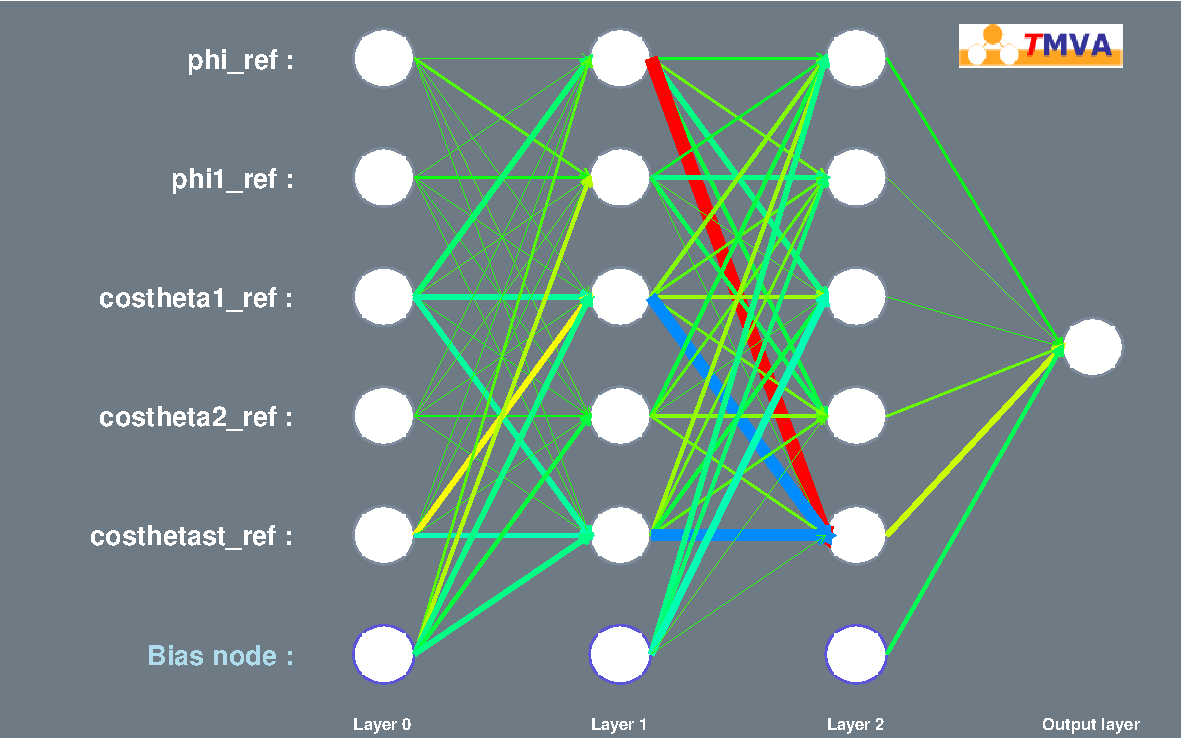
\includegraphics[width=0.8\linewidth]{images/plots/NN/nn_network_architecture}
\end{center}
\end{frame}

\begin{frame}{Neural Network Training and Testing}
\begin{center}
The trainings are done after preselection and additionally require at least one B-tagged Medium jet. (Trained on H 400 GeV)
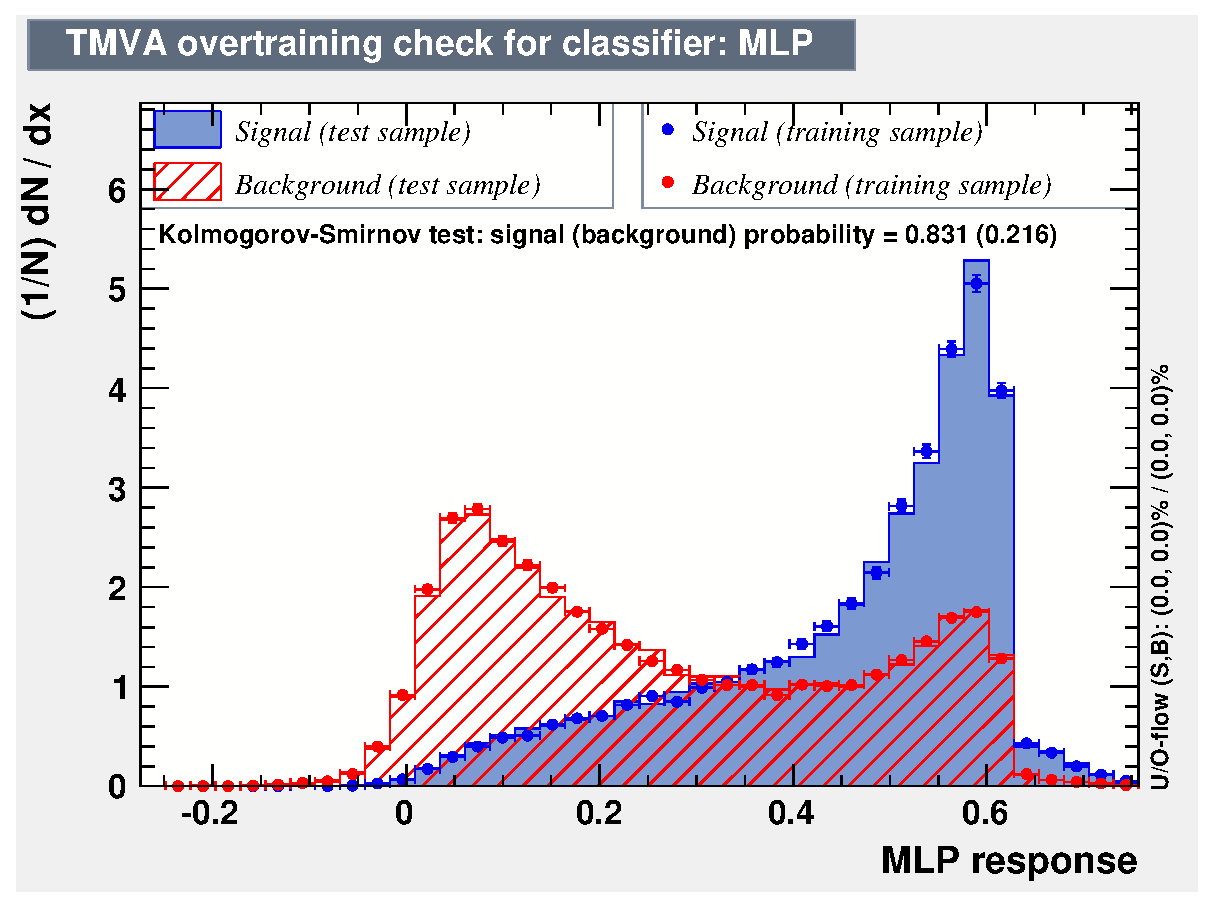
\includegraphics[width=0.7\linewidth]{images/plots/NN/MLP.eps}
%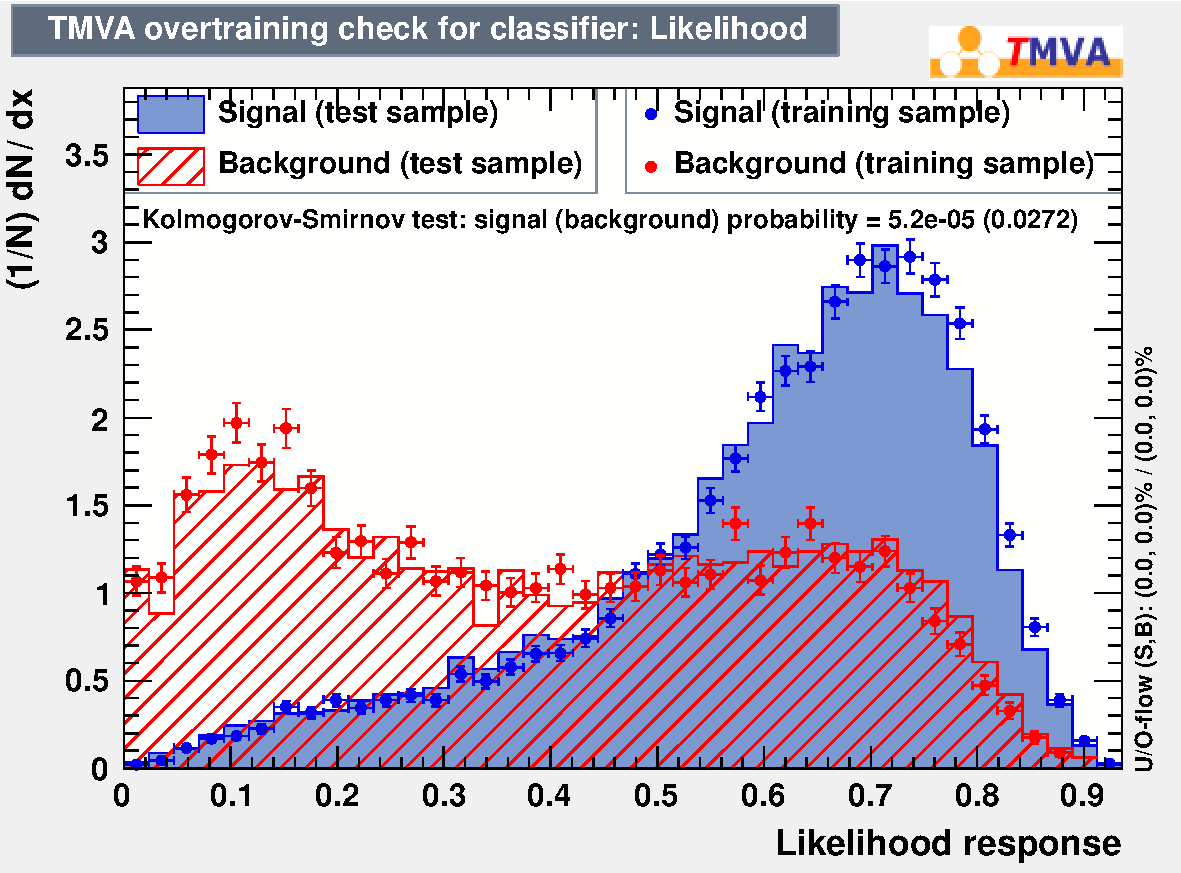
\includegraphics[width=0.5\linewidth]{images/plots/NN/Likelihood_TCHEM.pdf}
\end{center}
\end{frame}

%\begin{frame}{MLP}
%\begin{center}
%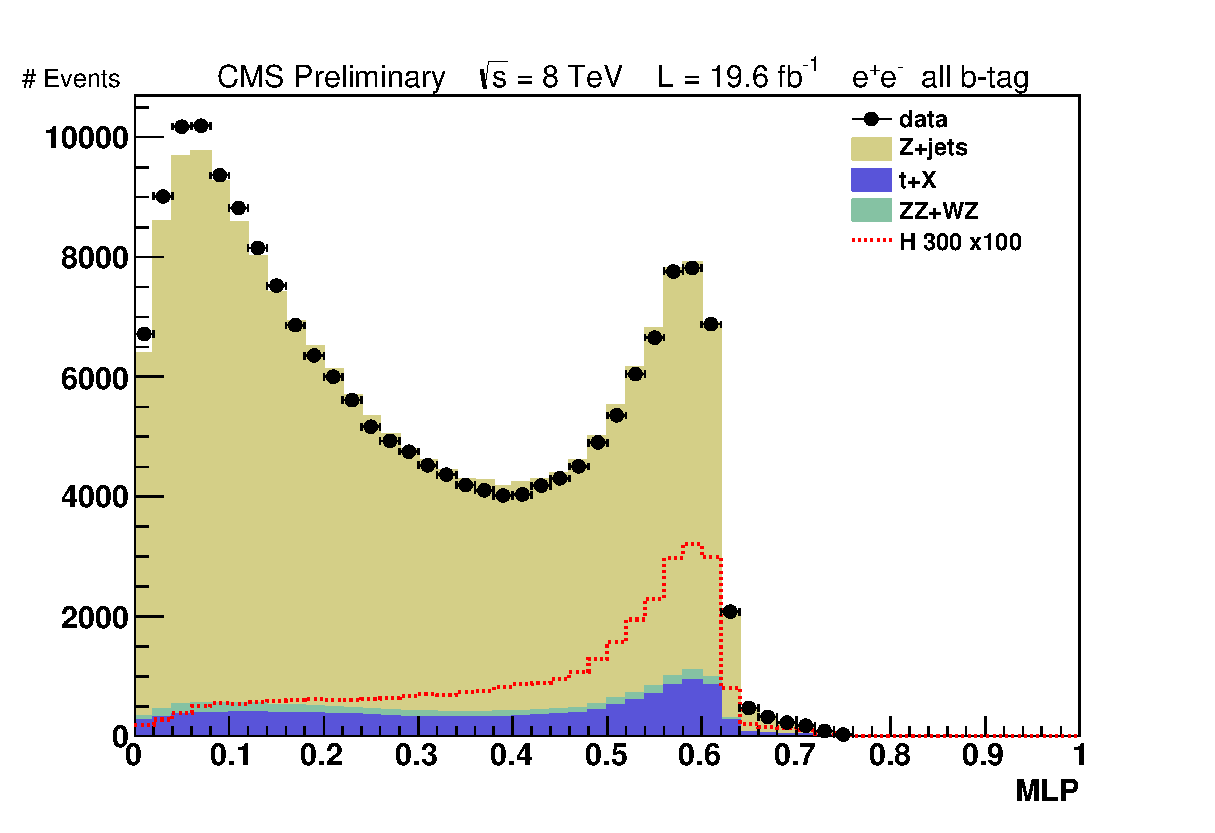
\includegraphics[width=0.49\textwidth]{images/preselection/el/MLP.eps}
%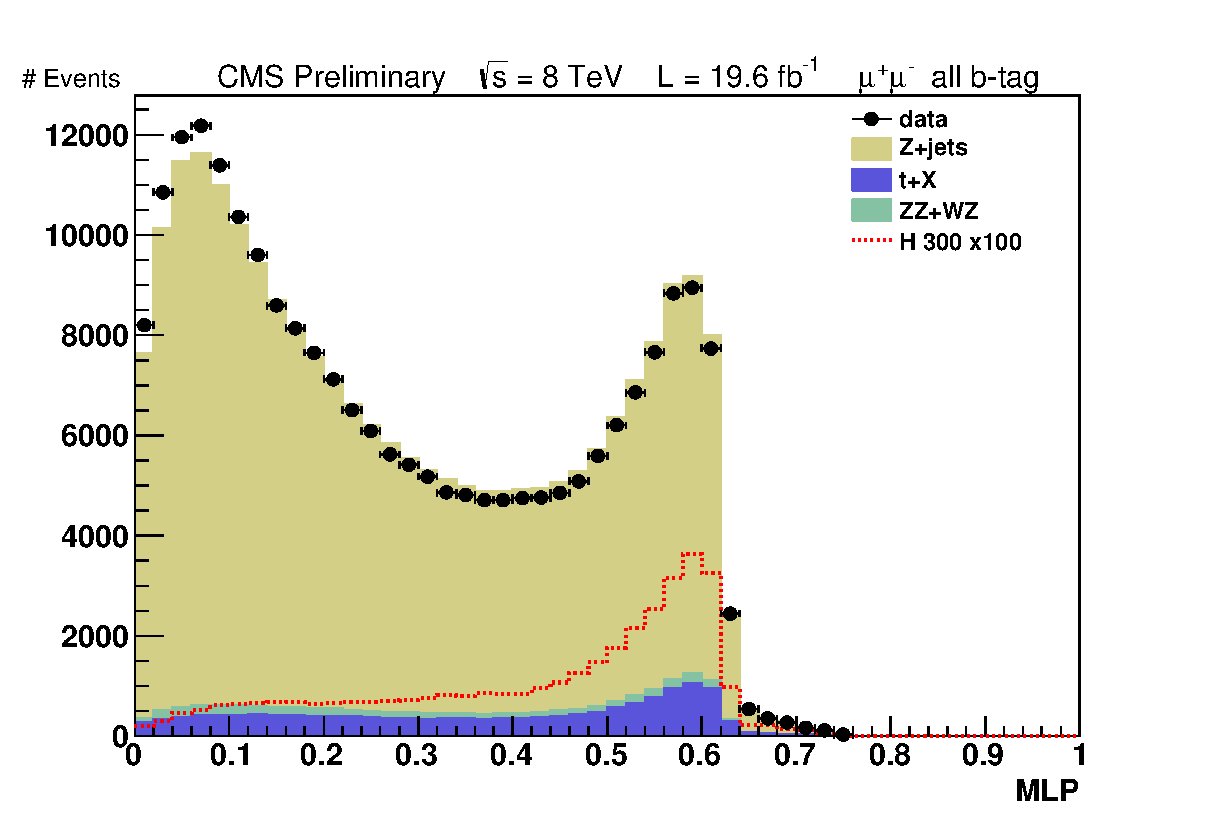
\includegraphics[width=0.49\textwidth]{images/preselection/mu/MLP.eps}\\
%\end{center}
%\end{frame}

\begin{frame}{MLP - In b-tag regions}
\begin{center}
Electrons (zero,one,two)\\
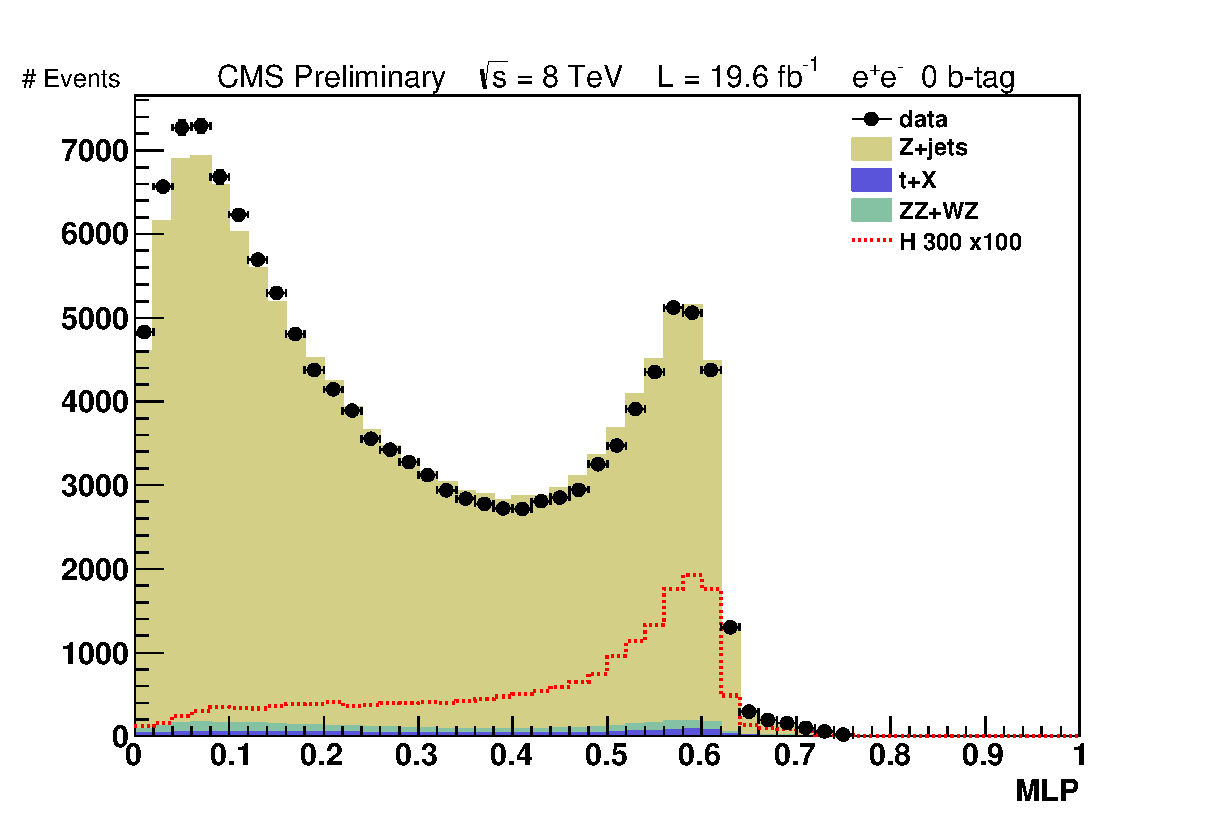
\includegraphics[width=0.33\textwidth]{images/preselection/0/el/MLP.eps}
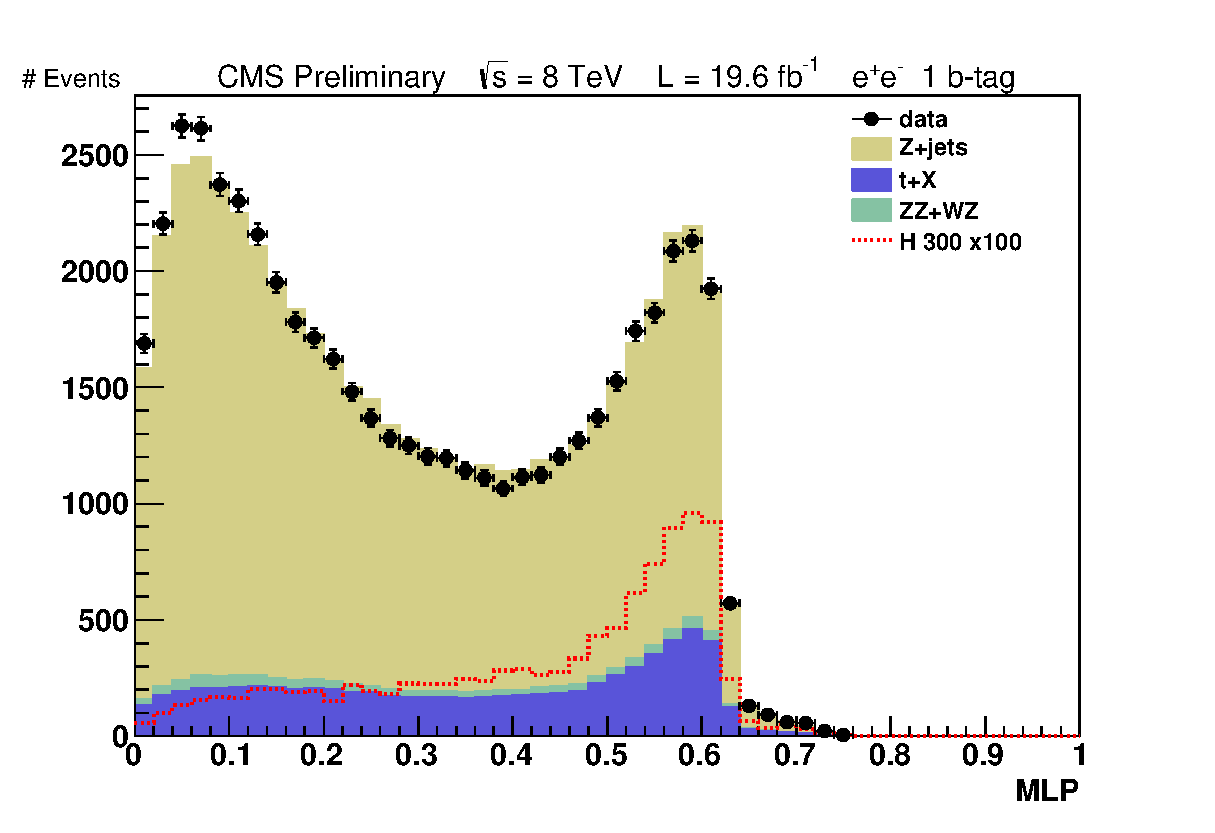
\includegraphics[width=0.33\textwidth]{images/preselection/1/el/MLP.eps}
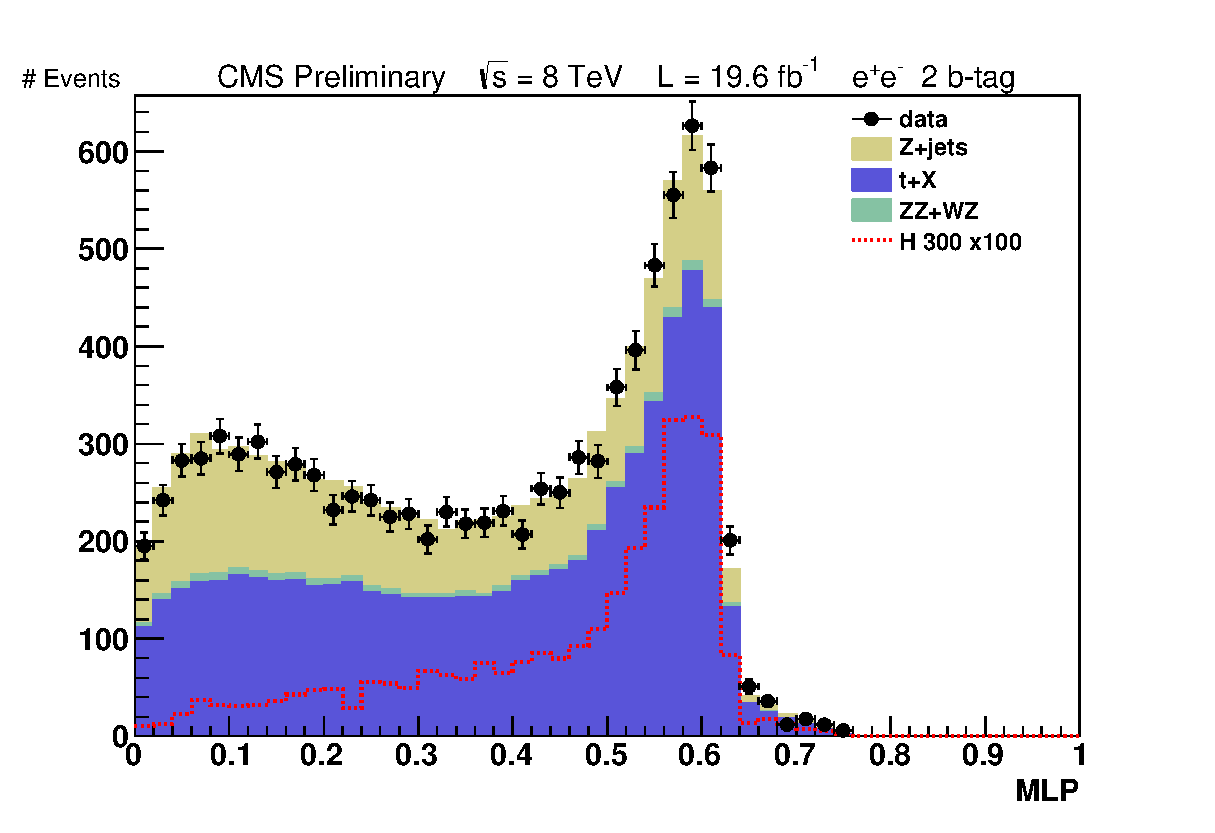
\includegraphics[width=0.33\textwidth]{images/preselection/2/el/MLP.eps}\\
Muons (zero,one,two)\\
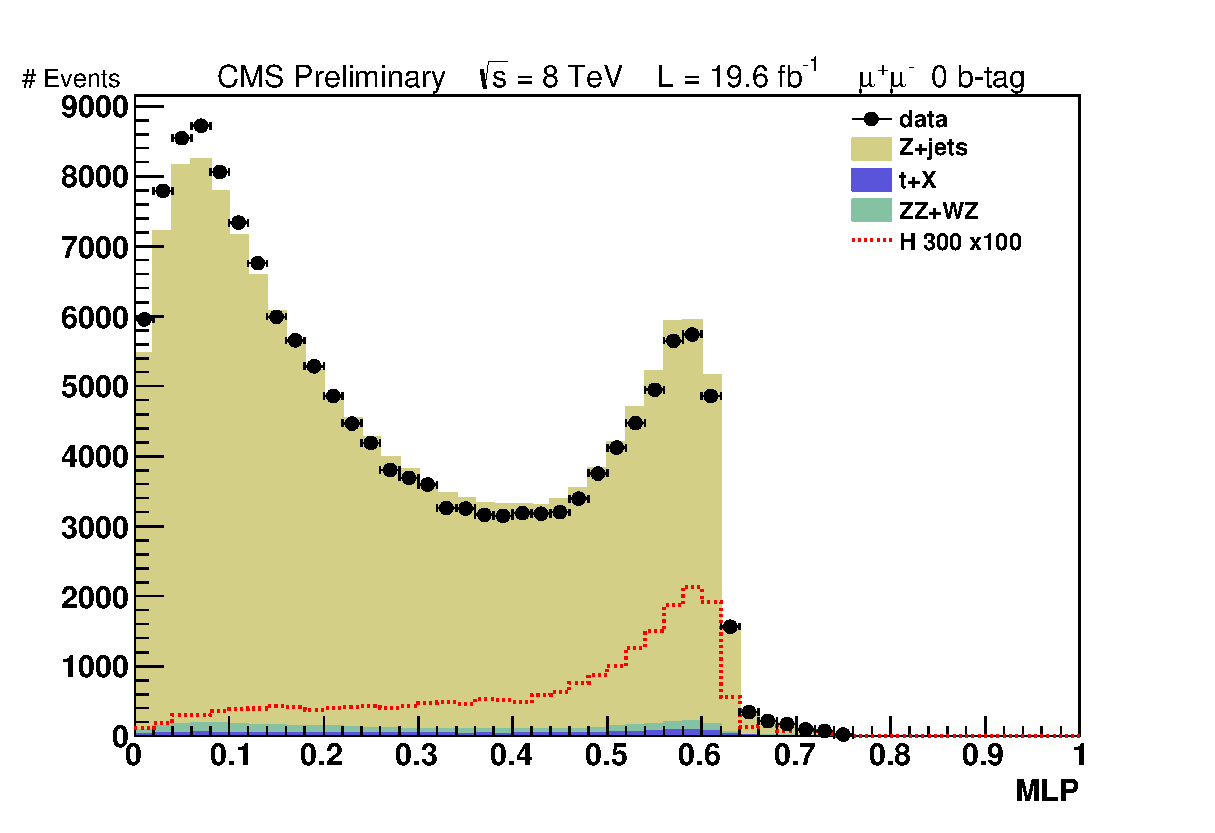
\includegraphics[width=0.33\textwidth]{images/preselection/0/mu/MLP.eps}
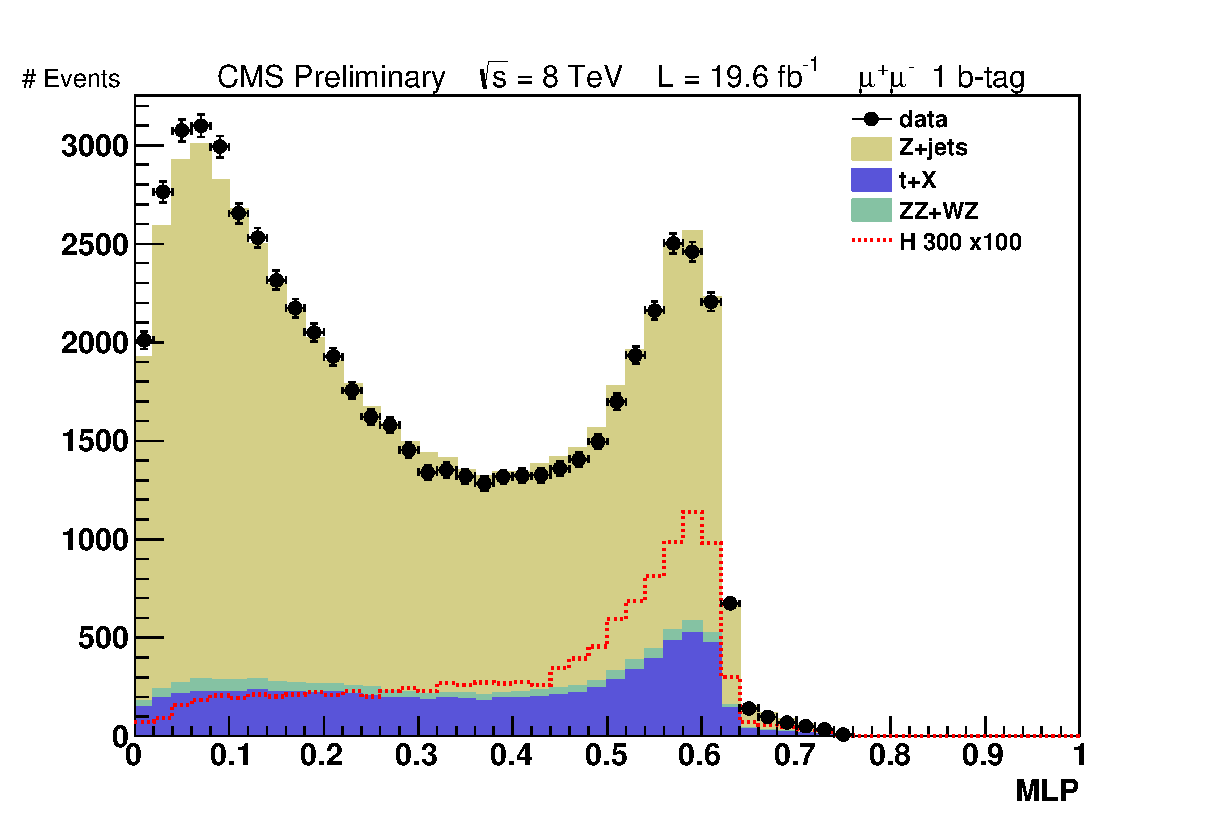
\includegraphics[width=0.33\textwidth]{images/preselection/1/mu/MLP.eps}
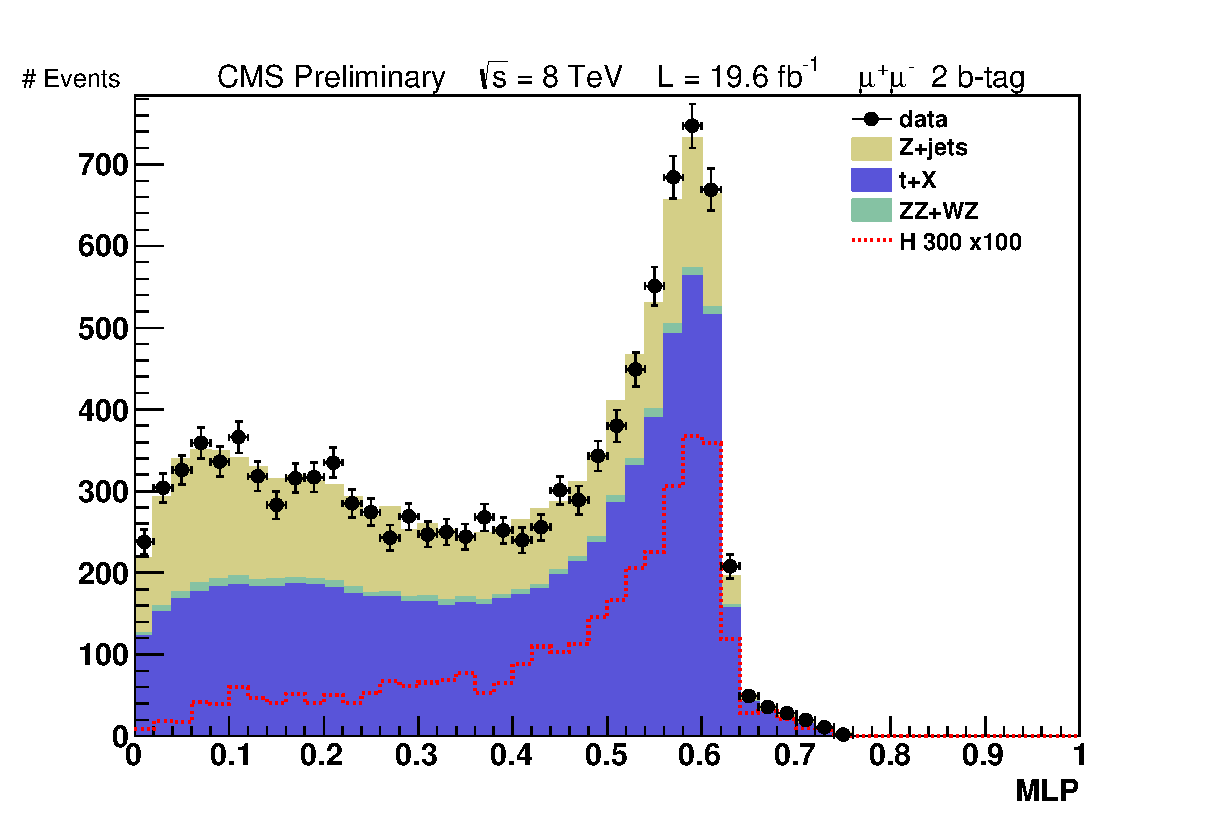
\includegraphics[width=0.33\textwidth]{images/preselection/2/mu/MLP.eps}\\
\end{center}
\end{frame}

%\begin{frame}{MLP - Many Higgs Masses}
%\begin{center}
%Electrons (zero,one,two)\\
%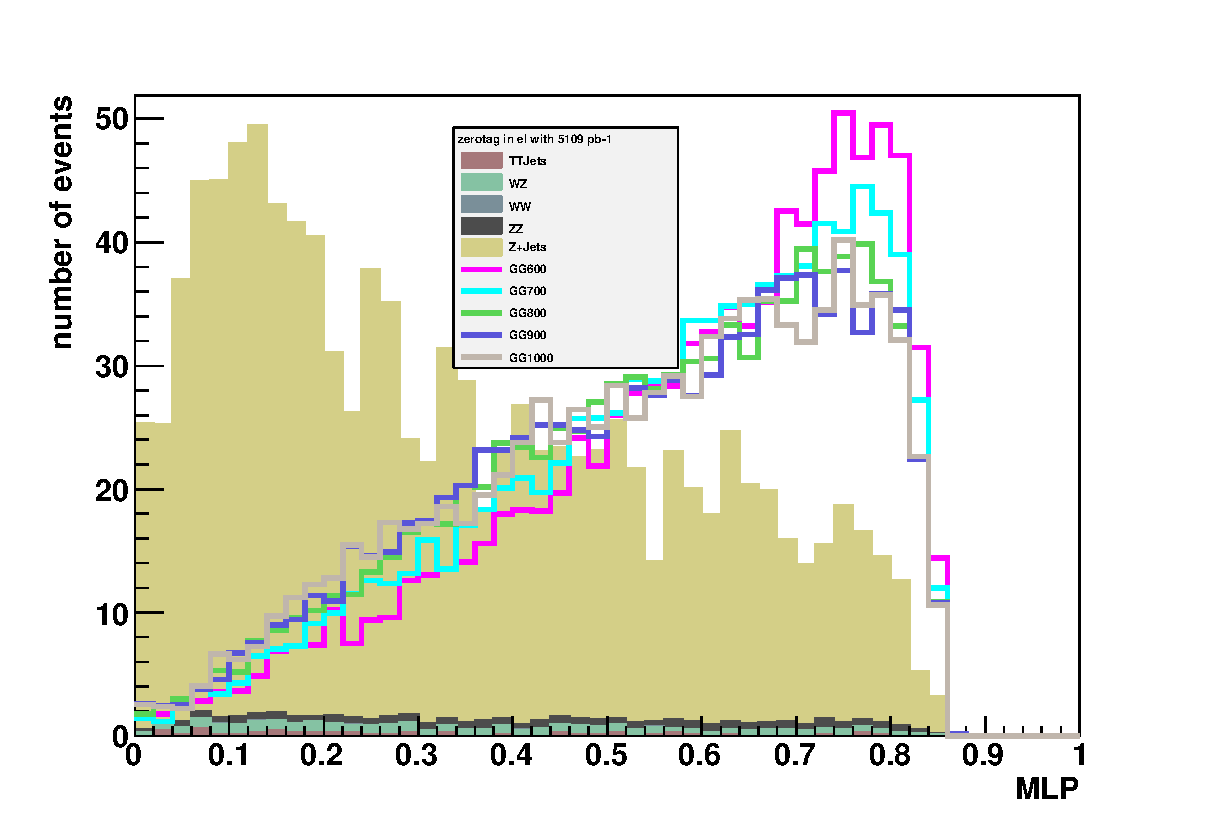
\includegraphics[width=0.33\textwidth]{images/mva_highmass/zero_MLP.eps}
%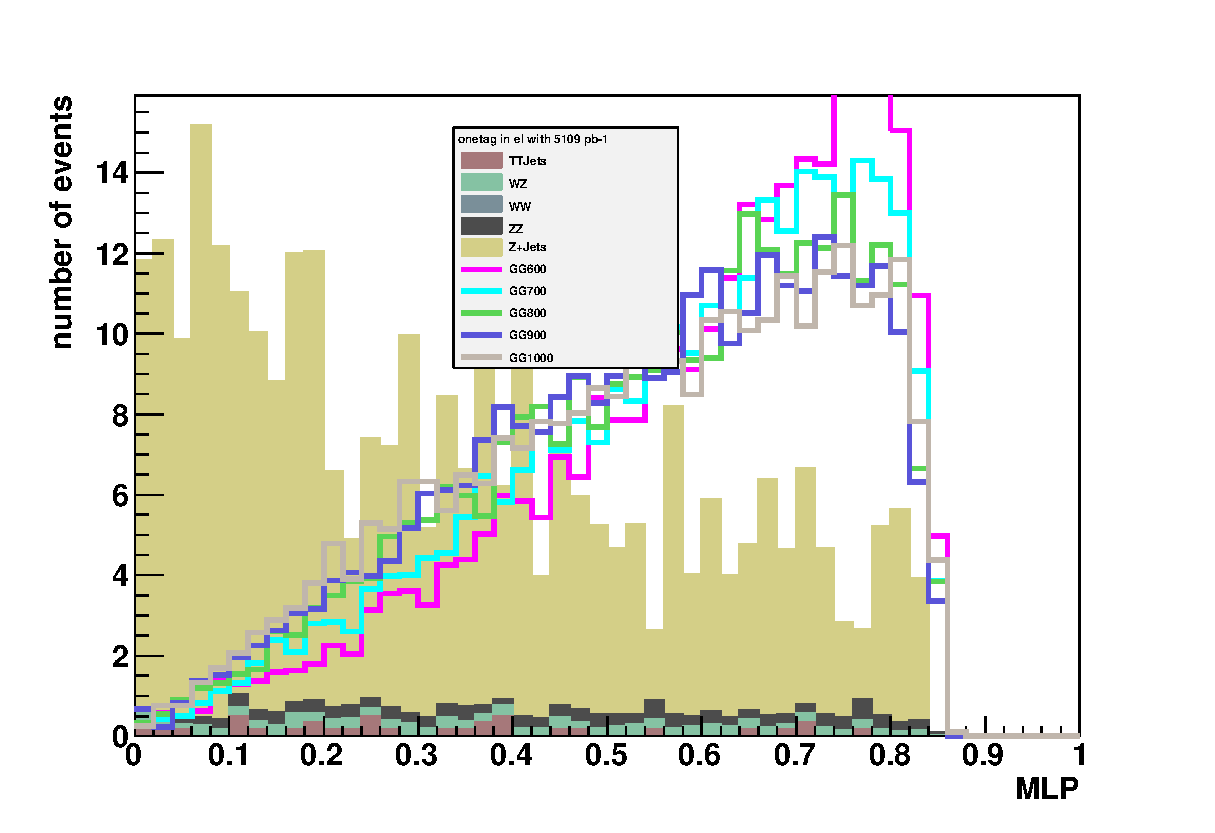
\includegraphics[width=0.33\textwidth]{images/mva_highmass/one_MLP.eps}
%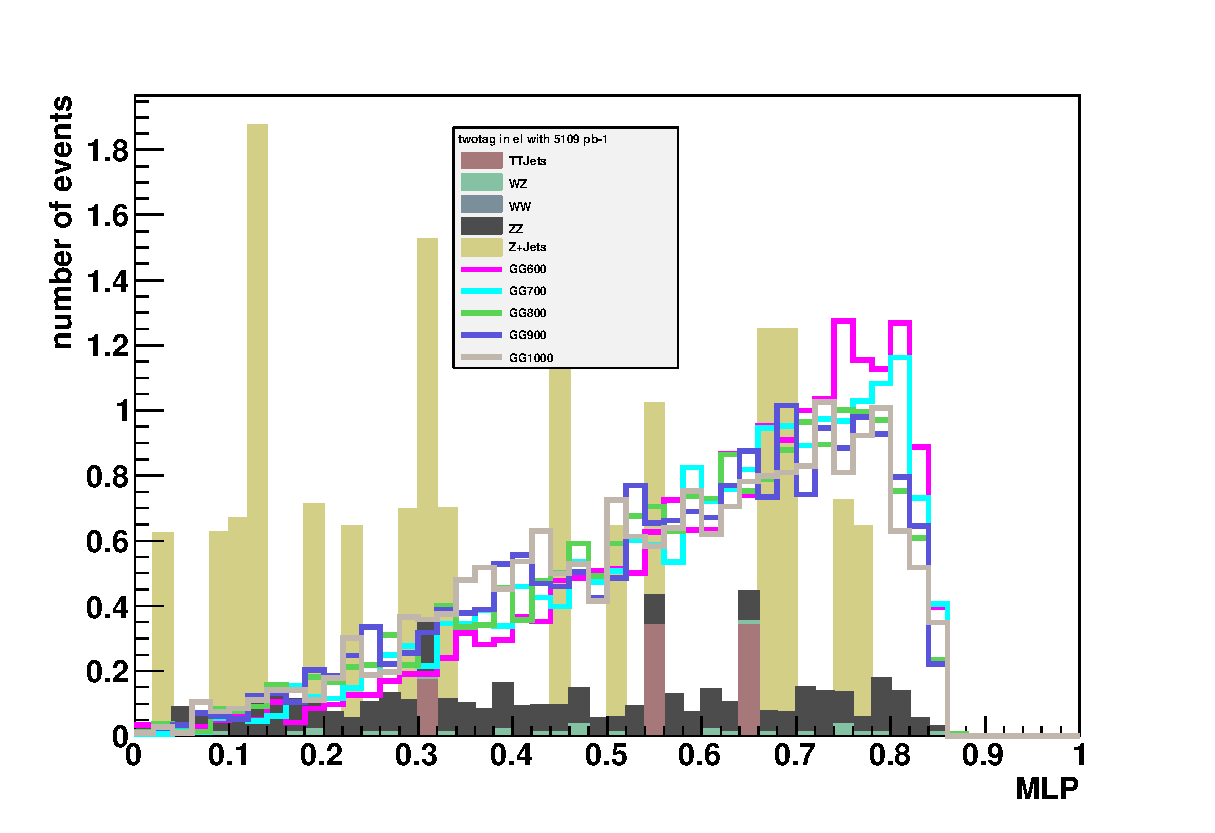
\includegraphics[width=0.33\textwidth]{images/mva_highmass/two_MLP.eps}\\
%Muons (zero,one,two)\\
%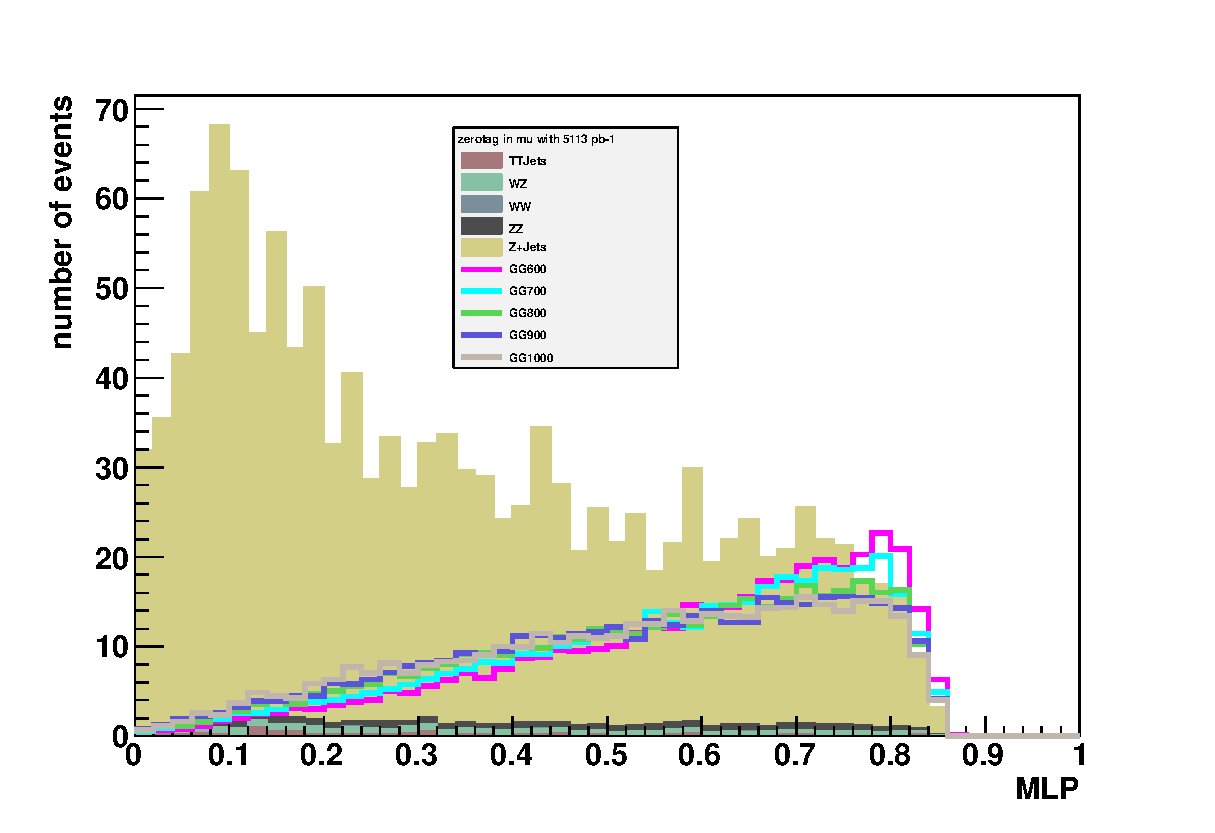
\includegraphics[width=0.33\textwidth]{images/mva_highmass/zero_mu_MLP.eps}
%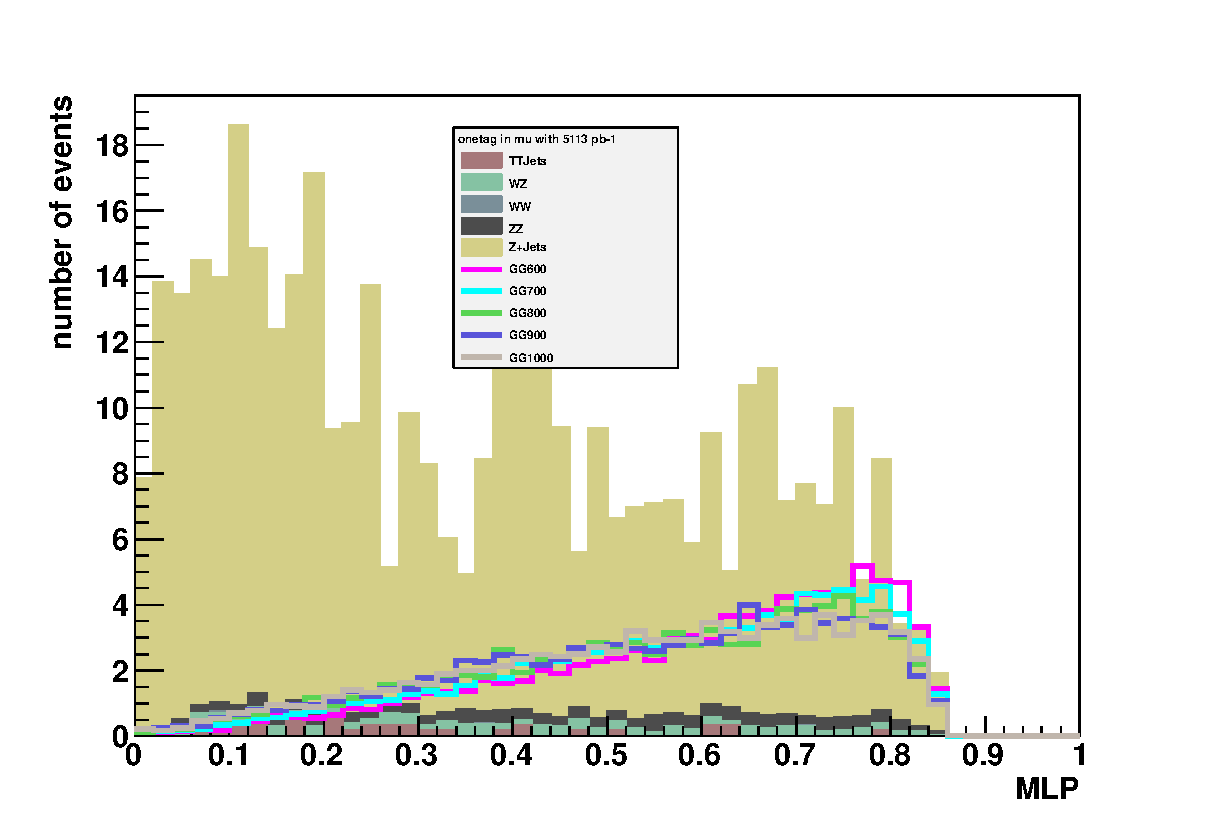
\includegraphics[width=0.33\textwidth]{images/mva_highmass/one_mu_MLP.eps}
%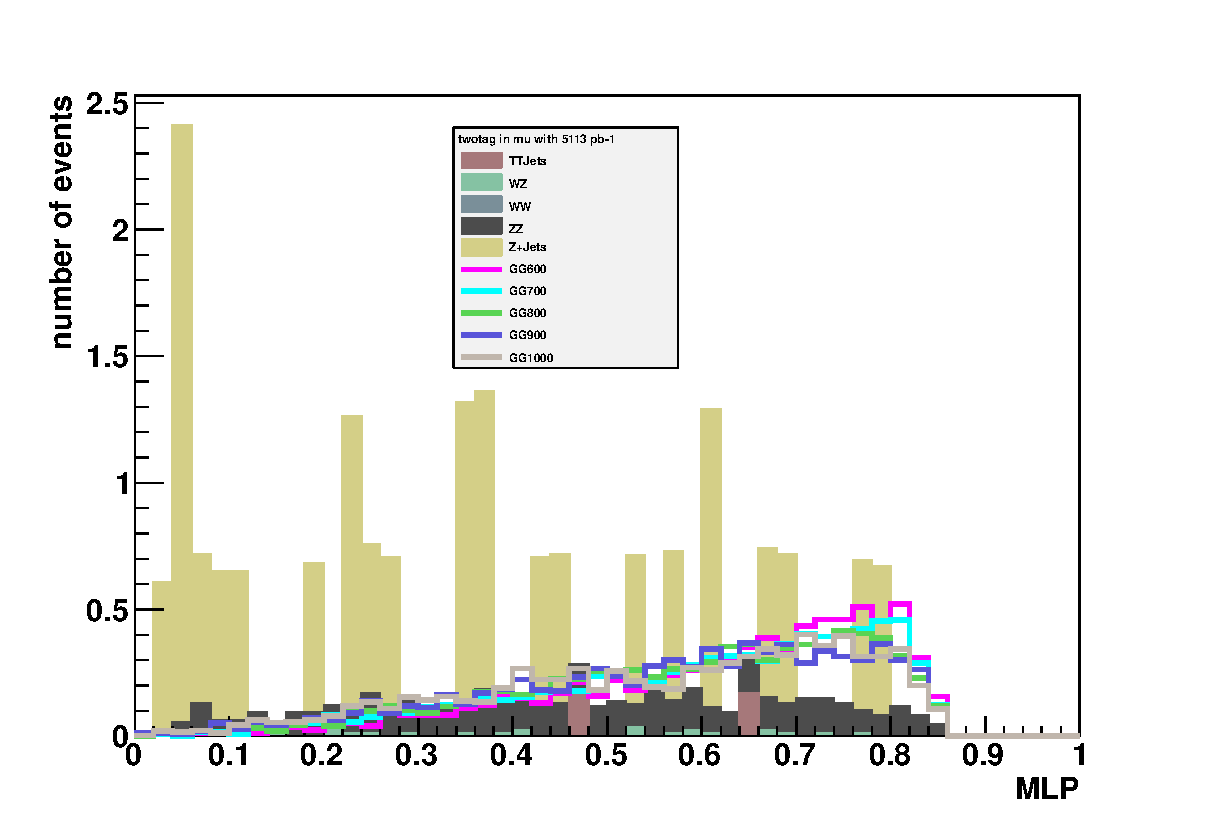
\includegraphics[width=0.33\textwidth]{images/mva_highmass/two_mu_MLP.eps}\\
%\end{center}
%\end{frame}

\begin{frame}{MLP vs Helicity LD}
\begin{center}
The working point is the background rejection point that we currently achieve in the two tag region in our analysis.
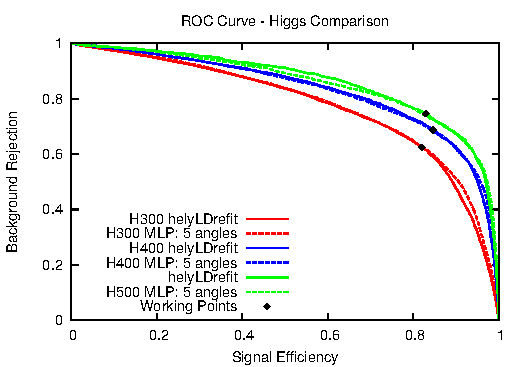
\includegraphics[width=0.7\linewidth]{images/plots/NN/pretag_ROC_wincut.pdf}
\end{center}
\end{frame}









\begin{frame}{$m_{ZZ}$ plots - Side Band Region}
  \begin{center}
    Electrons\\
    0-tag \hspace{7.5em} 1-tag \hspace{7.5em} 2-tag
  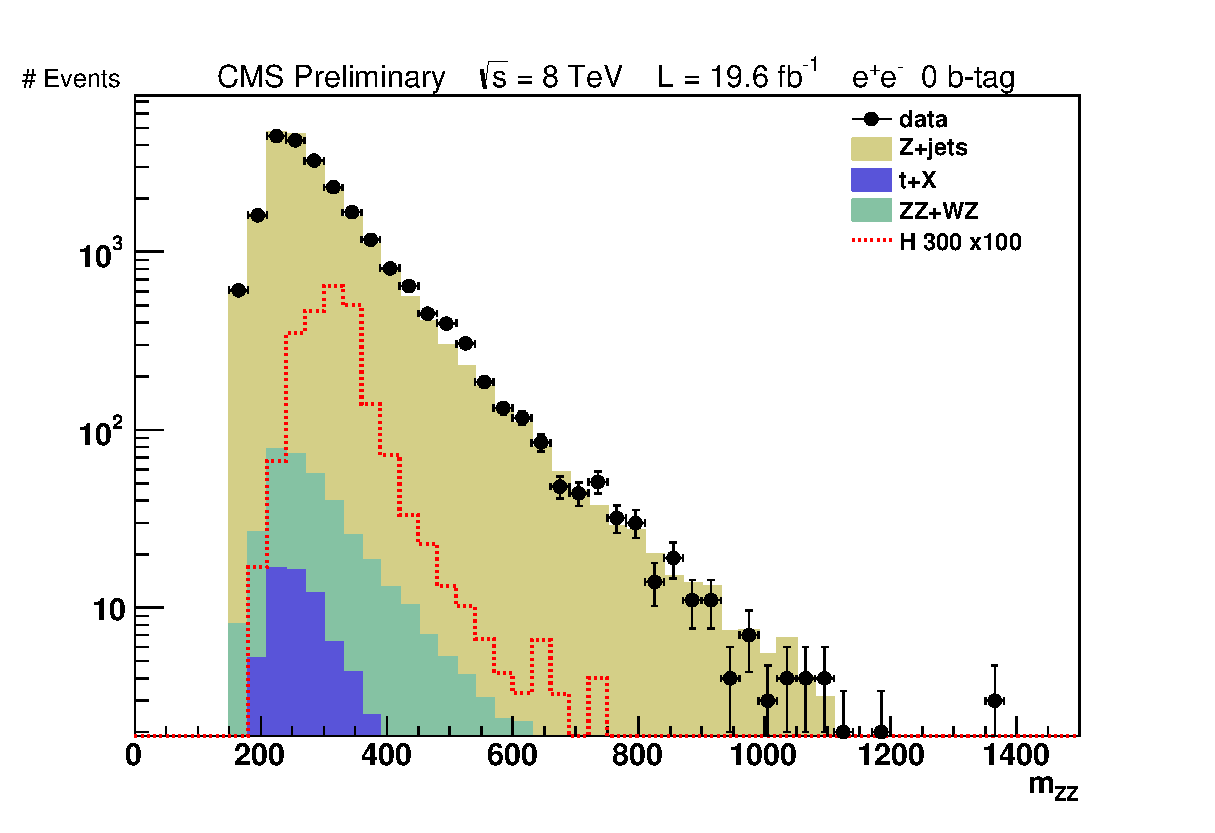
\includegraphics[width=0.33\textwidth]{images/preselection/0/el/mZZ_sideband_log.eps}
  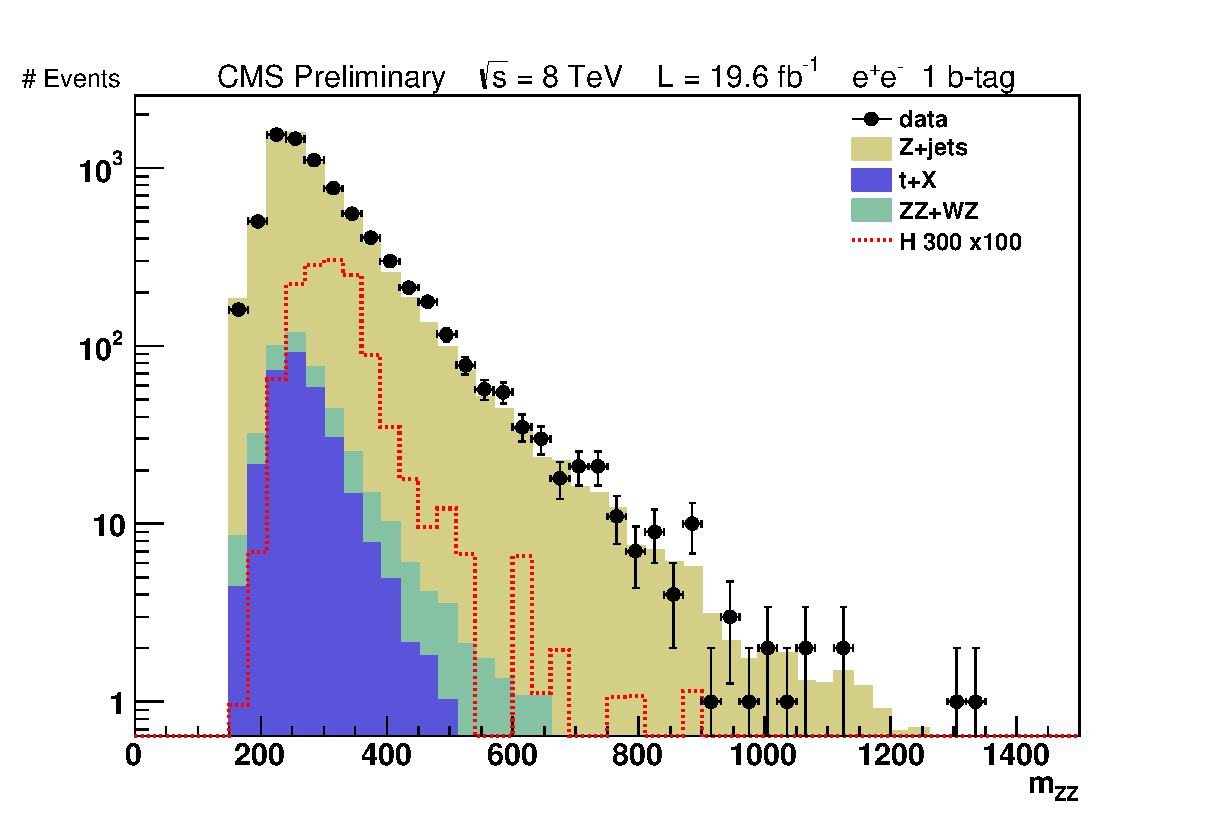
\includegraphics[width=0.33\textwidth]{images/preselection/1/el/mZZ_sideband_log.eps}
  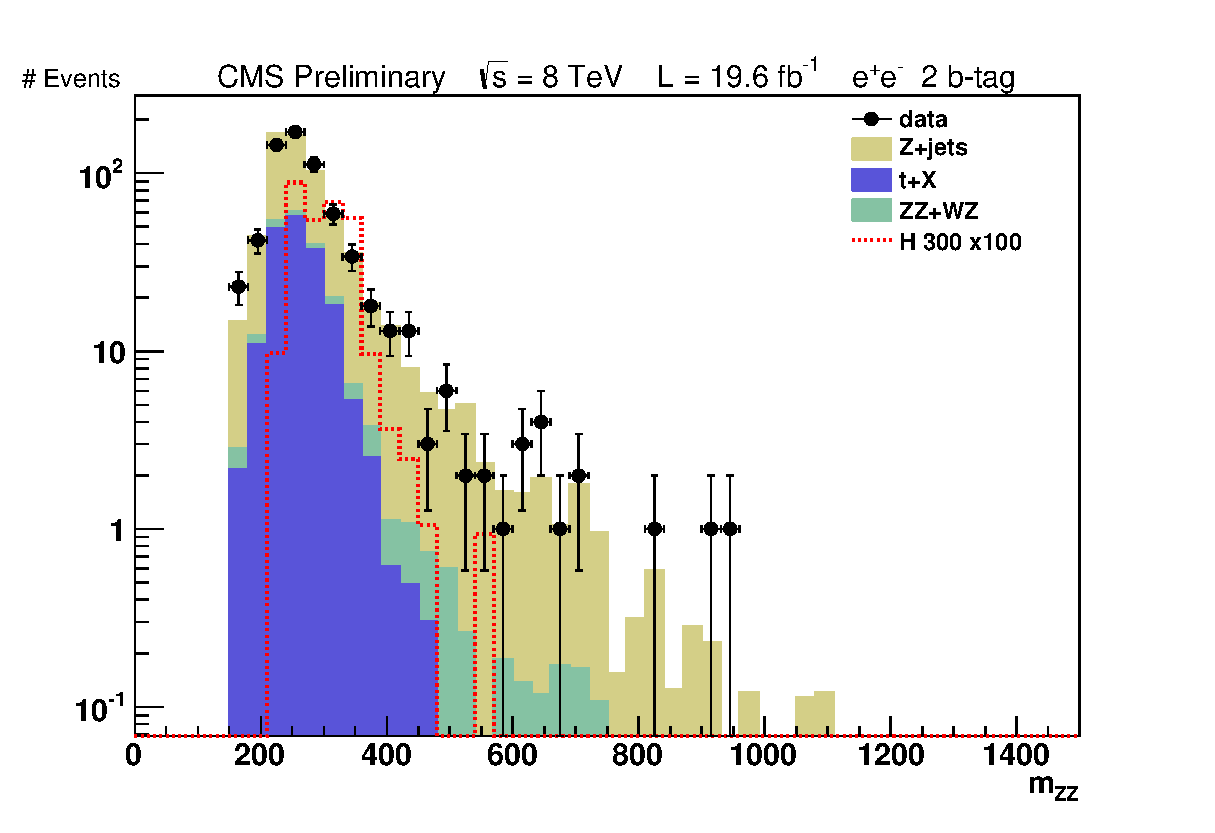
\includegraphics[width=0.33\textwidth]{images/preselection/2/el/mZZ_sideband_log.eps}\\
  Muons\\
    0-tag \hspace{7.5em} 1-tag \hspace{7.5em} 2-tag
  
  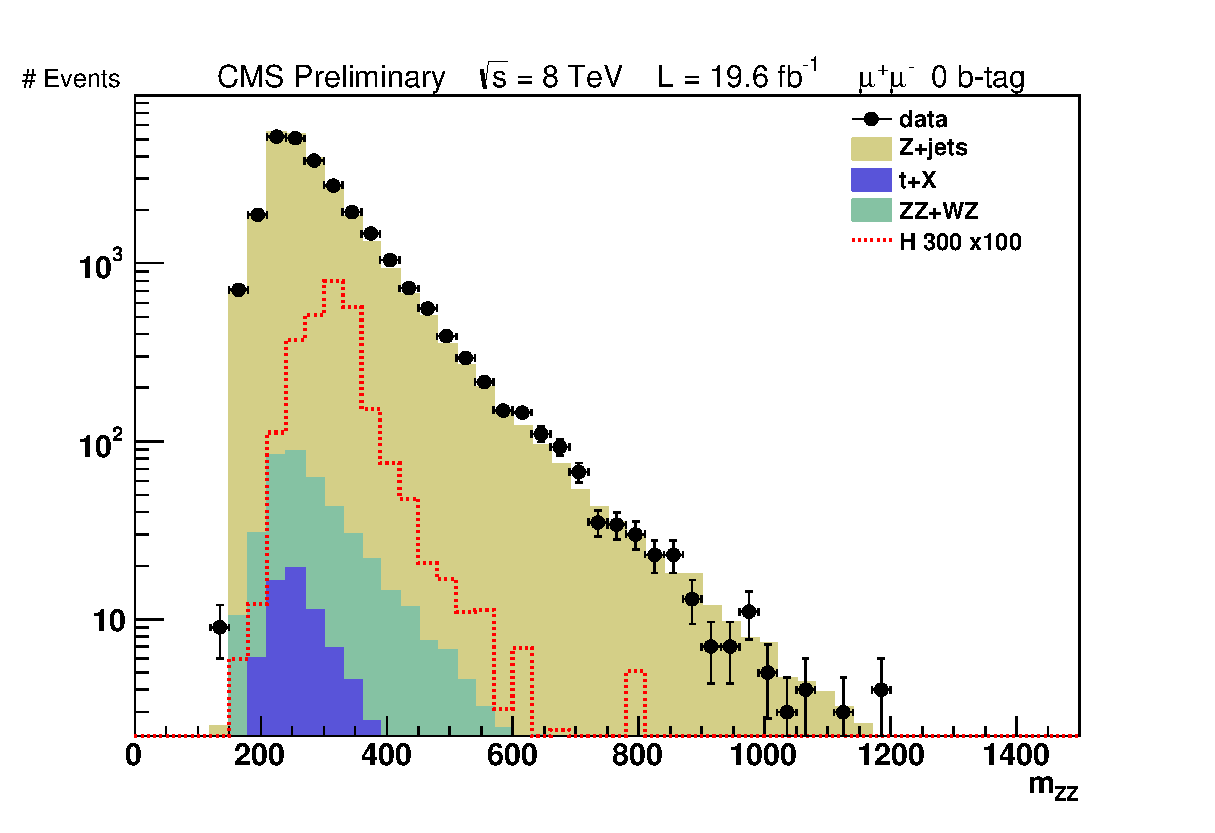
\includegraphics[width=0.33\textwidth]{images/preselection/0/mu/mZZ_sideband_log.eps}
  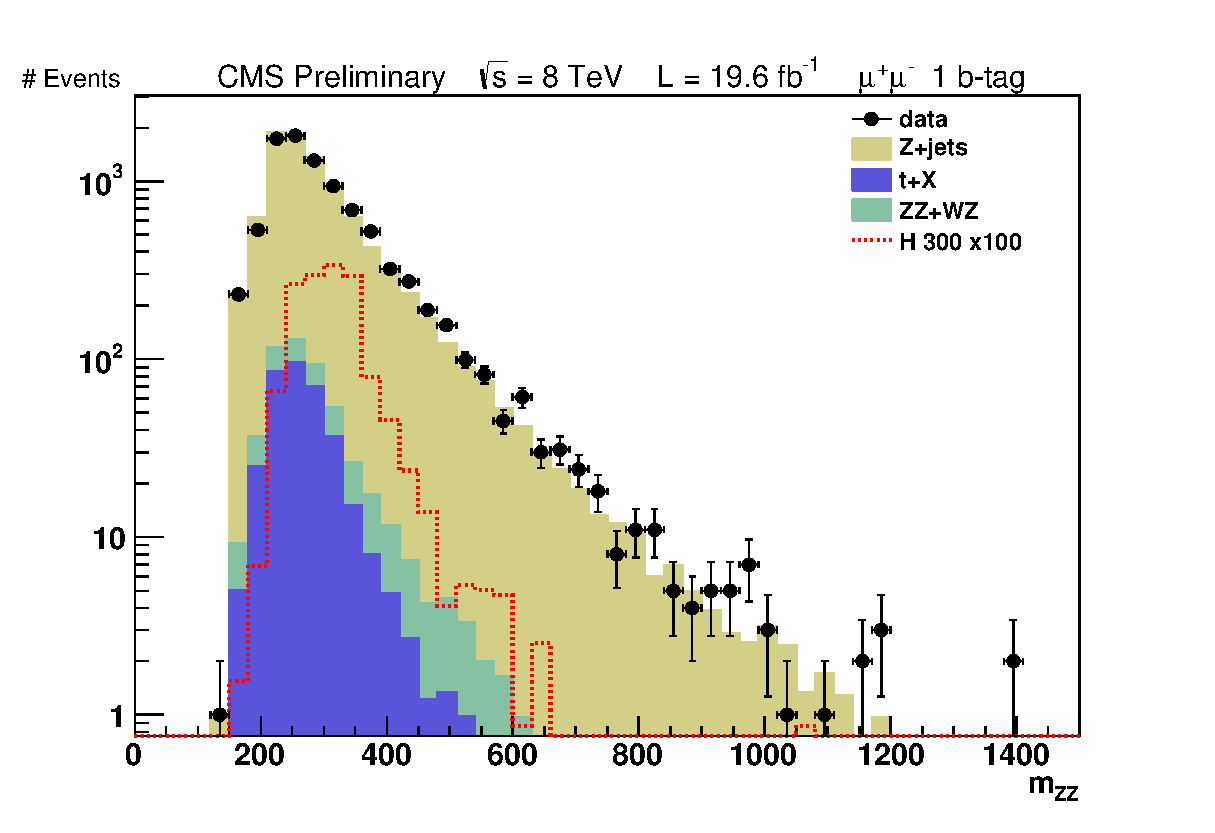
\includegraphics[width=0.33\textwidth]{images/preselection/1/mu/mZZ_sideband_log.eps}
  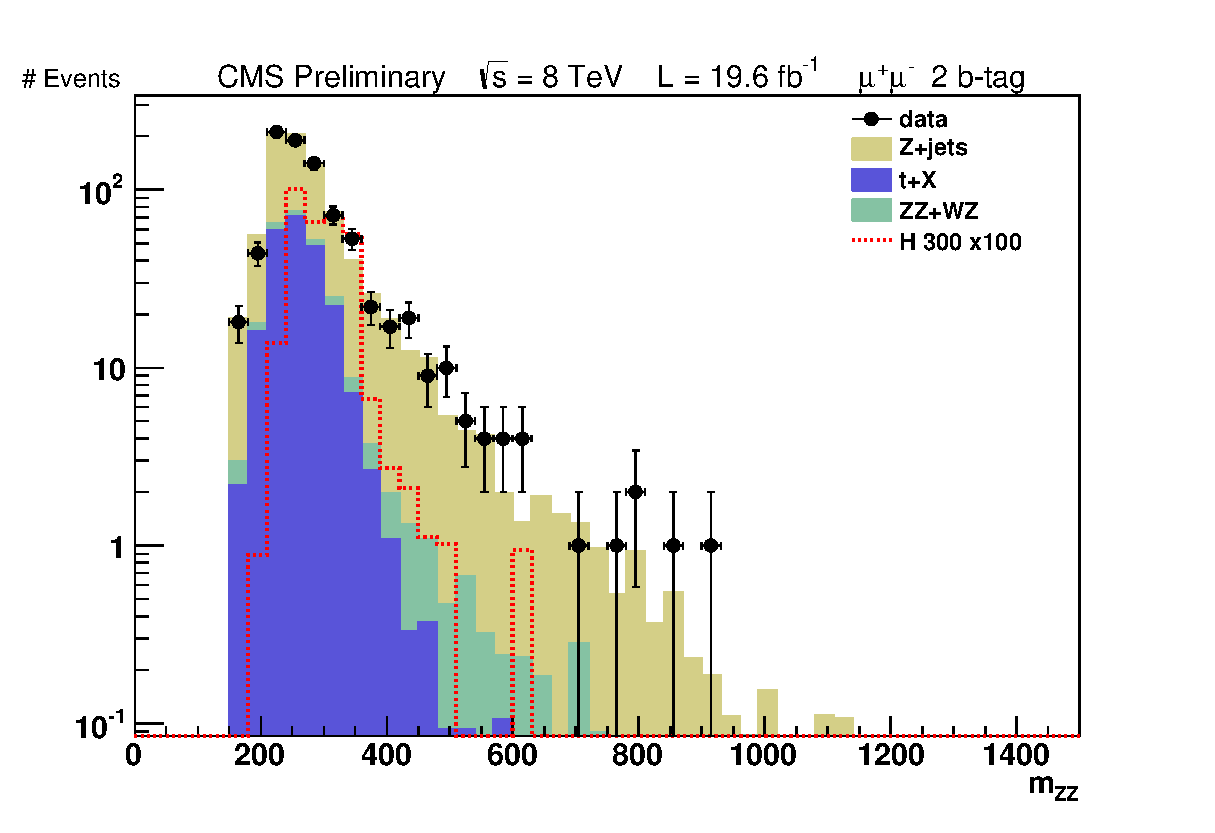
\includegraphics[width=0.33\textwidth]{images/preselection/2/mu/mZZ_sideband_log.eps}
  \end{center}
\end{frame}


\begin{frame}{Upper vs Lower Sideband}
\begin{center}
  We also have very similar performance between the upper and lower sidebands in the $m_{ZZ}$ distribution so we are able to use them together.
  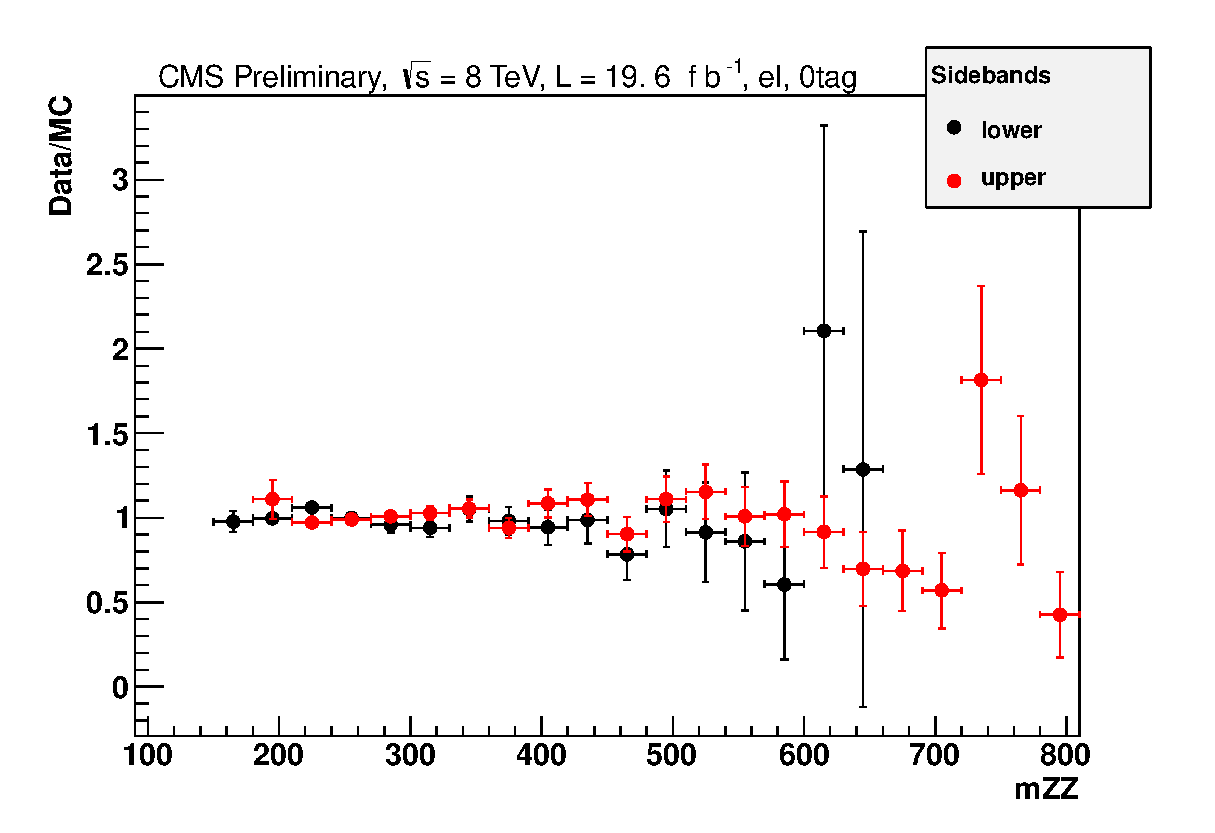
\includegraphics[width=0.5\textwidth]{images/sidebands/divide_el_2_0.eps}
   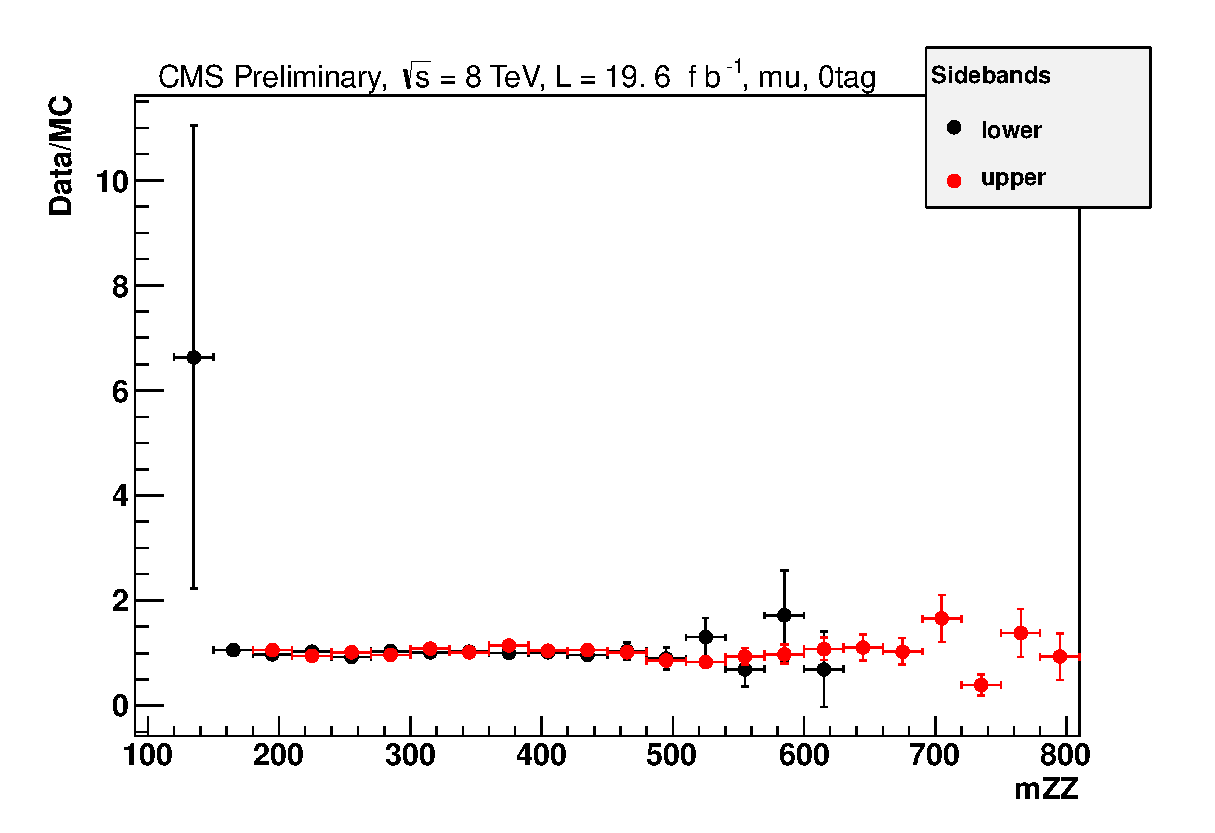
\includegraphics[width=0.5\textwidth]{images/sidebands/divide_mu_2_0.eps}
\end{center}
\end{frame}

\begin{frame}{Background Correction}
  \scriptsize
  \begin{itemize}
  \item
    We use the mjj sideband in data to get the normalization and a MC shape correction.

 % \begin{block}{}
 %   Number of background events in the signal region extrapolated from 
 % the side band region using the $\alpha(m_{ZZ})$ factor (as a function
 % of m$_{ZZ}$)
 % \begin{equation}
 %   N_{\rm bkg}(m_{ZZ})
 %   =N_{\rm sb}(m_{ZZ})\times\frac{N^{\rm MC}_{\rm bkg}(m_{ZZ})}{N^{\rm MC}_{\rm sb}(m_{ZZ})}
 %   =N_{\rm sb}(m_{ZZ})\times\alpha(m_{ZZ})
 % \end{equation}
 %  \end{block}
\item
  The fit is to a Fermi Function convoluted with a CrystallBall function
%  $\alpha$ is a flat factor while we wait for the exclusive samples
\end{itemize}

\begin{center}
%0-tag \vspace{7.5em} 1-tag \vspace{7.5em} 2-tag\\
    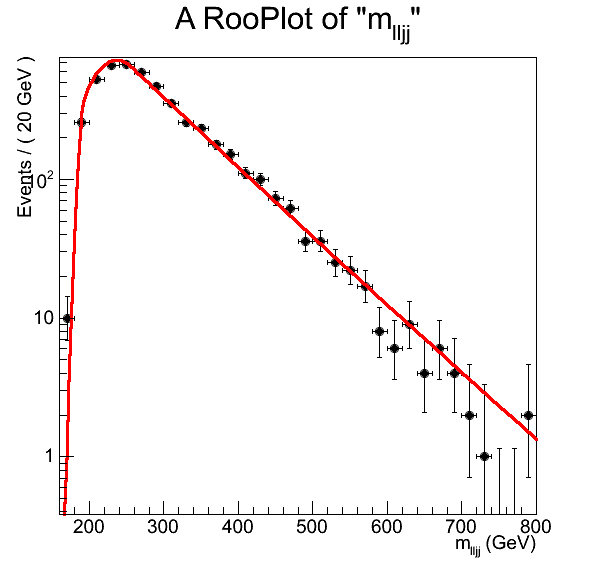
\includegraphics[width=0.3\textwidth]{images/fromDani/mZZ_sidebandsDATA_alpha_0btag_ALL_log.png}
    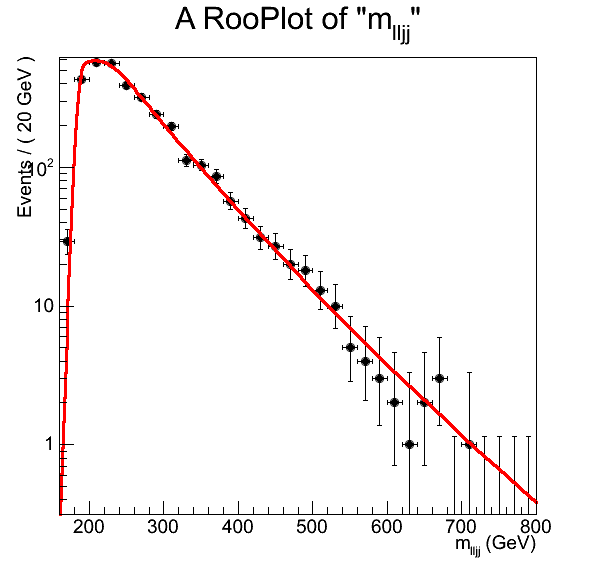
\includegraphics[width=0.3\textwidth]{images/fromDani/mZZ_sidebandsDATA_alpha_1btag_ALL_log.png}
    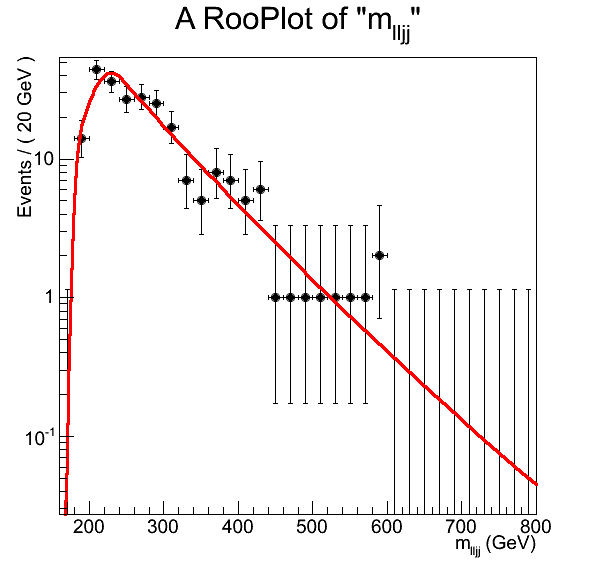
\includegraphics[width=0.3\textwidth]{images/fromDani/mZZ_sidebandsDATA_alpha_2btag_ALL_log.png}\\
0-tag \hspace{10.5em} 1-tag \hspace{10.5em} 2-tag
\end{center}

\end{frame}


%\begin{frame}{Selection Requirements}
%\begin{center}
%\begin{tabular}{|l|c|c|c|}
%\hline
% observable      &   0 $b$-tag   &   1 $b$-tag  &   2 $b$-tag  \\ \hline
%btag & none & JPL & JPL \& JPM \\ \hline
%helicity LD  &  \multicolumn{3}{|c|}{> 0.5}   \\ 
%missing $E_{T}$ significance &  \multicolumn{3}{|c|}{< 10}   \\ 
%$m_{jj}$  &  \multicolumn{3}{|c|}{[71,111] GeV/$c^{2}$}   \\ 
%$m_{ll}$  &  \multicolumn{3}{|c|}{[76,106] GeV/$c^{2}$}   \\ \hline
%$p_{T}(l^{\pm})$ & \multicolumn{3}{|c|}{> 40/20 GeV/c} \\
%$p_{T}(jets)$ & \multicolumn{3}{|c|}{> 30 GeV/c} \\
%|$\eta$|$(l^{\pm})$ & \multicolumn{3}{|c|}{$e^{\pm}$ < 2.5, $\mu^{\pm}$ < 2.4} \\
%|$\eta$|(jets) & \multicolumn{3}{|c|}{< 2.4} \\ \hline
%\multicolumn{4}{|c|}{lepton quailty} \\
%\multicolumn{4}{|c|}{jet quailty} \\ \hline
%\end{tabular}
%\end{center}
%\end{frame}


\begin{frame}{Tag and Probe}
\begin {itemize}
  \item
    Method to use Z boson to calculate efficincy of Data and Monte Carlo.
  \item
    One lepton is ``good'' (tag) and the other is used for the calculations(probe).
  \item
    Compairing Monte Carlo to data gives us Scale Factors.
\end{itemize}
\begin{center}
SuperCluster to GSF Electron\\
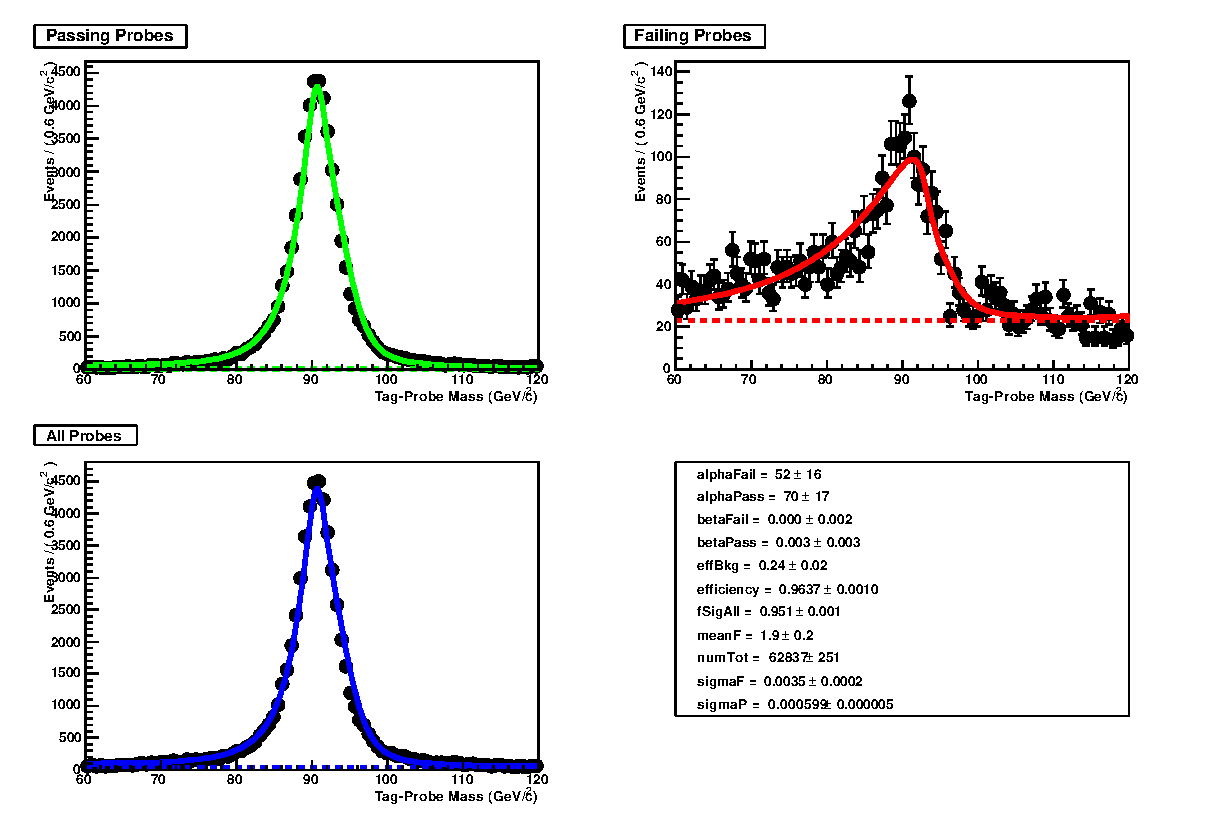
\includegraphics[width=0.49\textwidth]{images/SC_fit.eps}
\end{center}
\end{frame}


%\begin{frame}{Triggers}
%  \begin{columns}
%    \begin{column}{0.4\textwidth}
%      \begin{itemize}
%      \item
%        \footnotesize Muons
%        \begin{itemize}
%          \scriptsize
%        \item
%          HLT\_Mu17\_Mu8
%        \item
%          HLT\_Mu17\_TkMu8
%        \end{itemize}
%      \end{itemize}
%    \end{column}
%    \begin{column}{0.3\textwidth}
%      \begin{center}
%        {\tiny Electron Leg 8 GeV WPLoose to HLT}
%        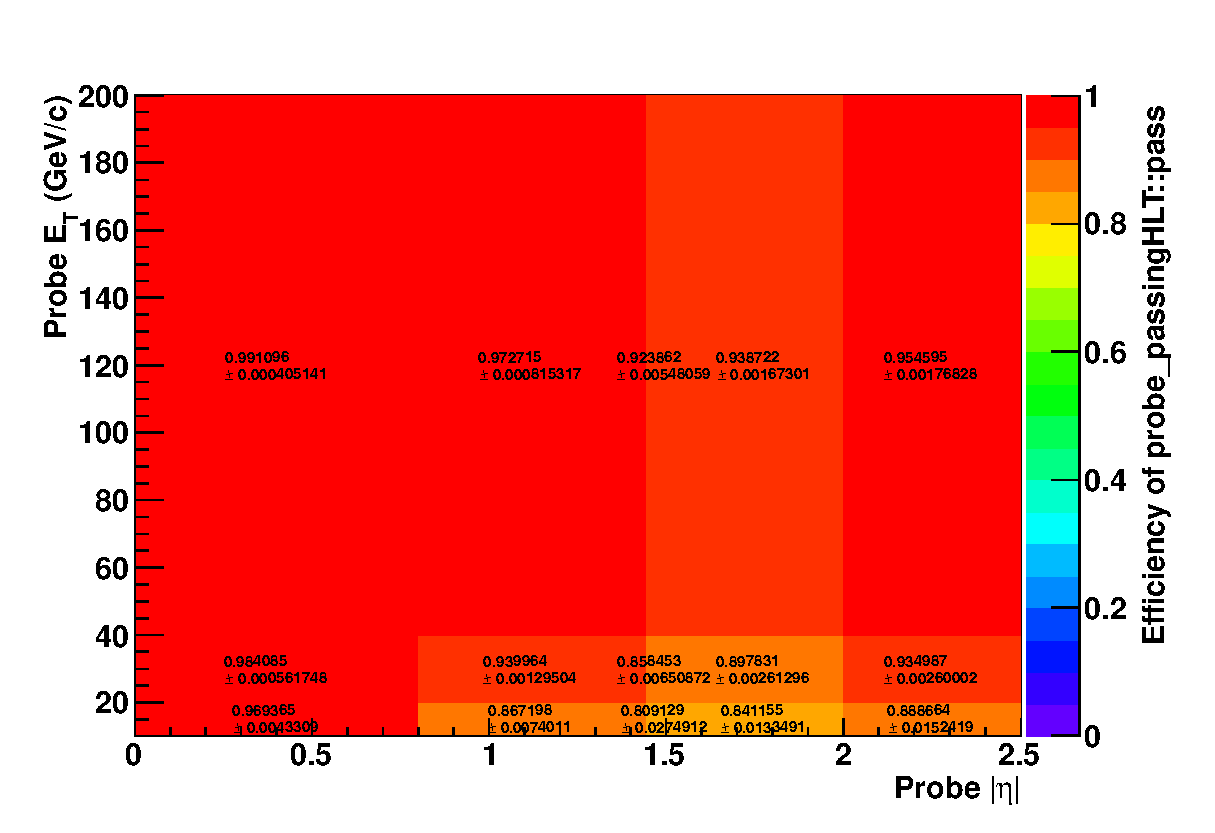
\includegraphics[width=0.99\textwidth]{images/ZJets_8.eps}
%      \end{center}
%    \end{column}
%    \begin{column}{0.3\textwidth}
%      \begin{center}
%      {\tiny Electron Leg 17 GeV WPLoose to HLT}
%      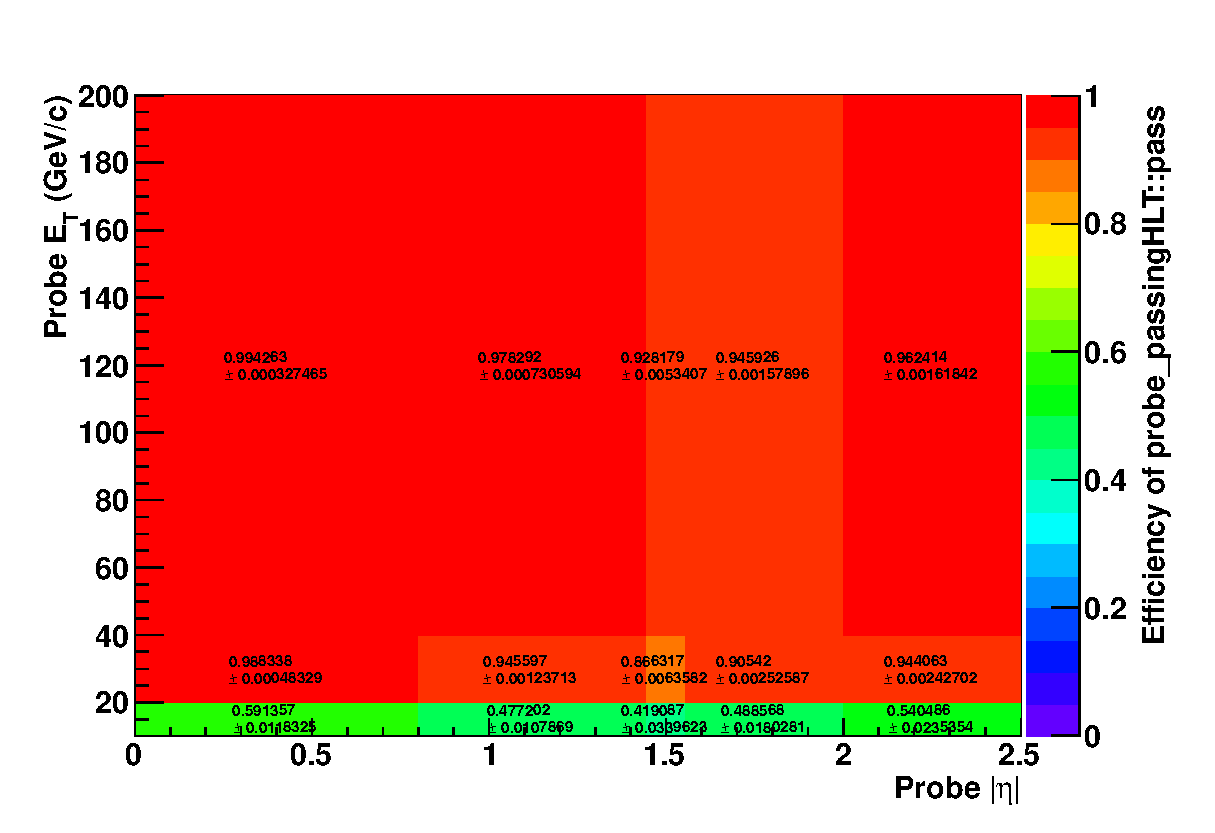
\includegraphics[width=0.99\textwidth]{images/ZJets_17.eps}
%      \end{center}
%    \end{column}
%  \end{columns}
%  \begin{columns}
%    \begin{column}{1.0\textwidth}
%  \begin{itemize}
%  \item
%    \footnotesize  Electrons
%    \begin{itemize}
%      \tiny
%    \item
%      HLT\_Ele17\_CaloIdT\_CaloIsoVL\_TrkIdVL\_TrkIsoVL \_Ele8\_CaloIdT\_CaloIsoVL\_TrkIdVL\_TrkIsoVL
%    \end{itemize}
%  \item
%    \footnotesize EMu (for backround estimation and analysis checks)
%    \begin{itemize}
%      \scriptsize
%    \item
%      Mu8\_Ele17\_CaloIdT\_CaloIsoVL
%    \item
%      Mu17\_Ele8\_CaloIdT\_CaloIsoVL\_TrkIdVL\_TrkIsoVL
%    \end{itemize}
%  \end{itemize}
%  \end{column}
%    \begin{column}{0.0\textwidth}
%    \end{column}
%  \end{columns}
%\vspace{2em}
%We are using the POG provided scale factors for electrons and computing the WP to HLT ourselves. 
%\end{frame}














%\begin{frame}{Efficiency Fit}
%The signal efficiency as a function of the Higgs mass is fitted to a polynomial in order to be estimatated for those Higgs mass hypothesis where no Monte-Carlo sample is available
%\begin{center}
%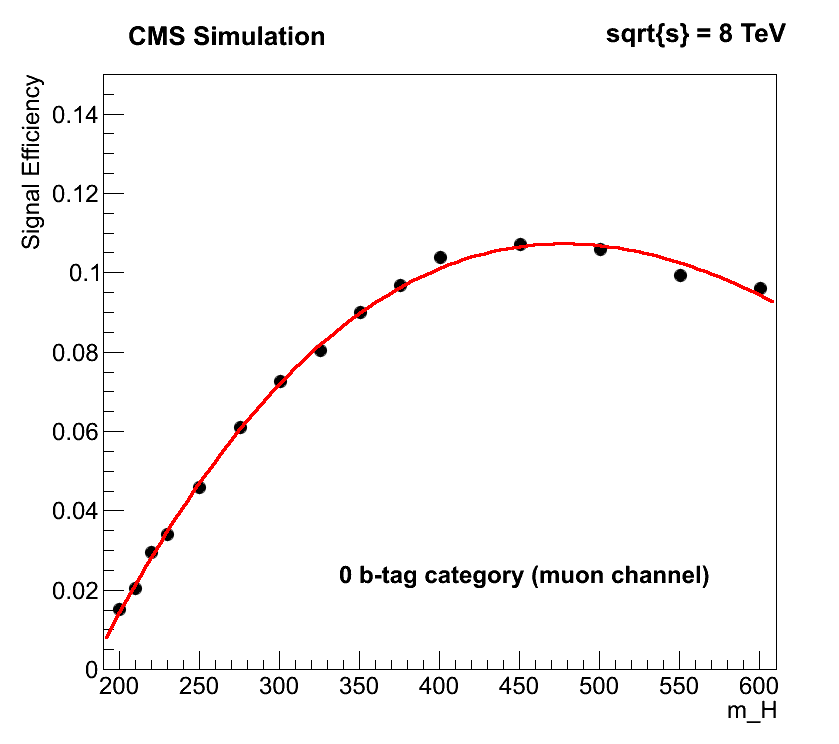
\includegraphics[width=0.3\textwidth]{images/plots/effFit_MU_0btag.png}
%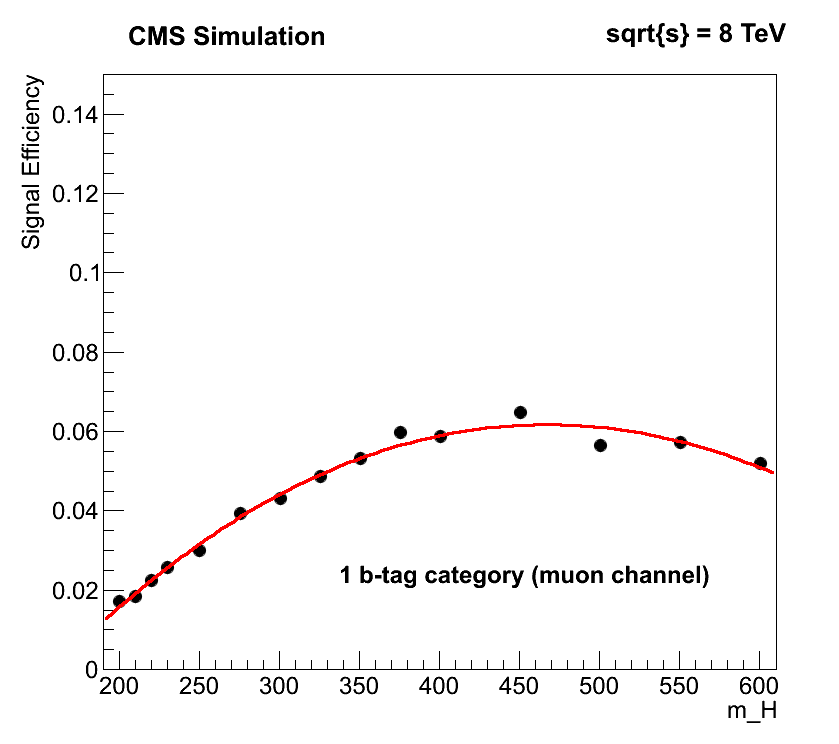
\includegraphics[width=0.3\textwidth]{images/plots/effFit_MU_1btag.png}
%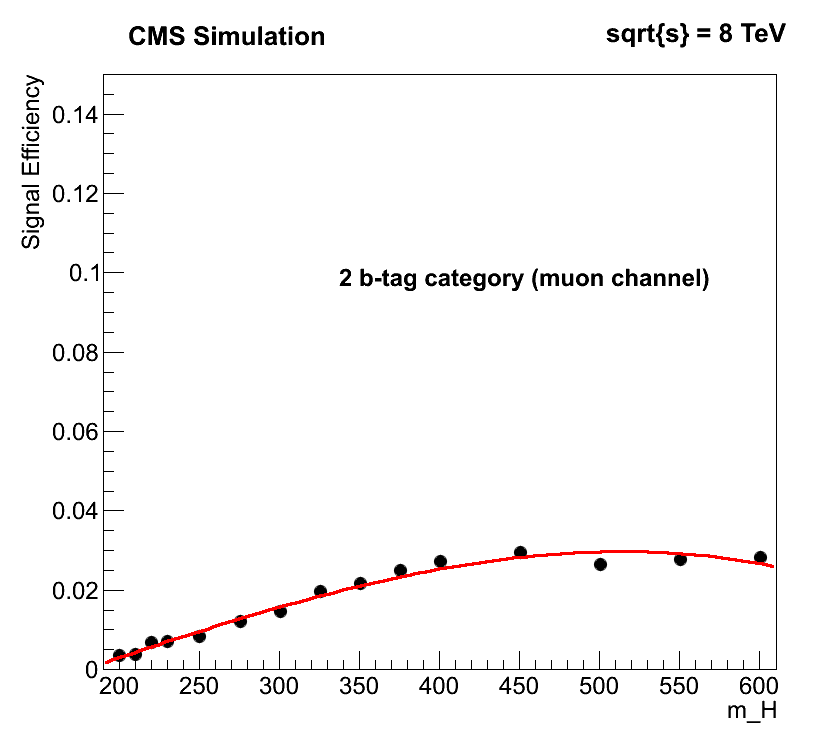
\includegraphics[width=0.3\textwidth]{images/plots/effFit_MU_2btag.png}
%\\

%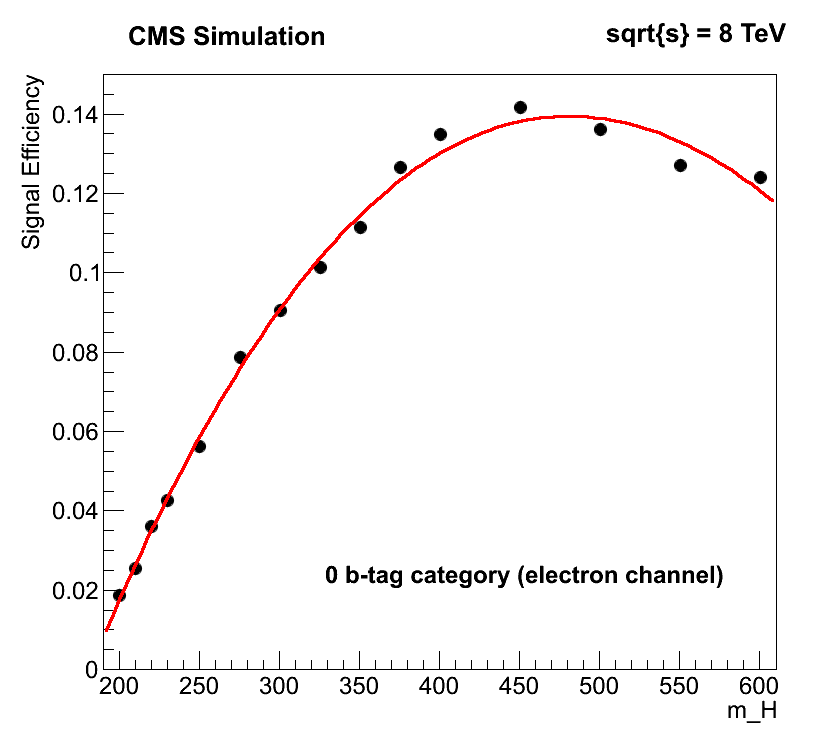
\includegraphics[width=0.3\textwidth]{images/plots/effFit_ELE_0btag.png}
%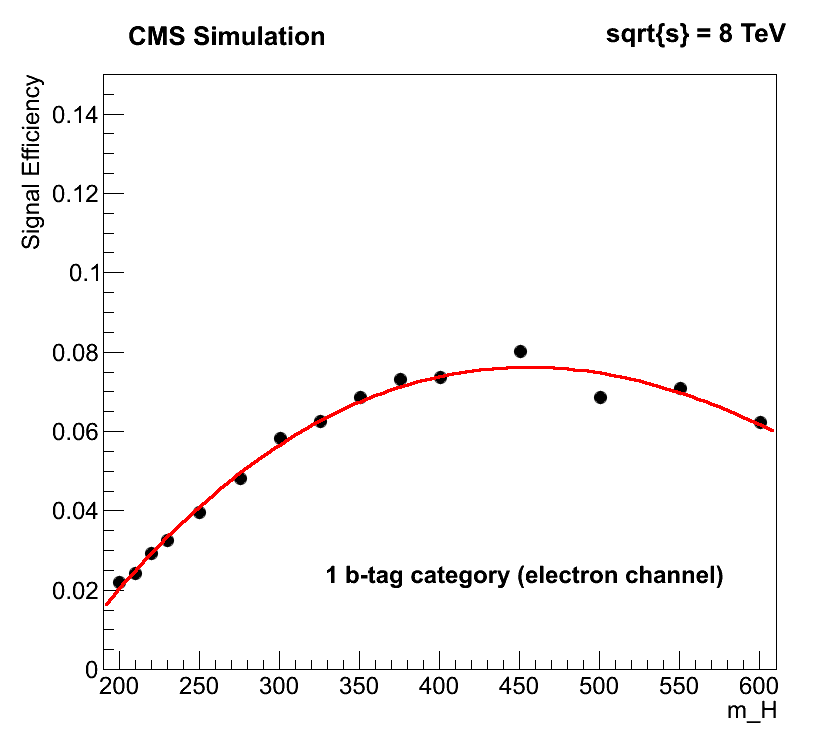
\includegraphics[width=0.3\textwidth]{images/plots/effFit_ELE_1btag.png}
%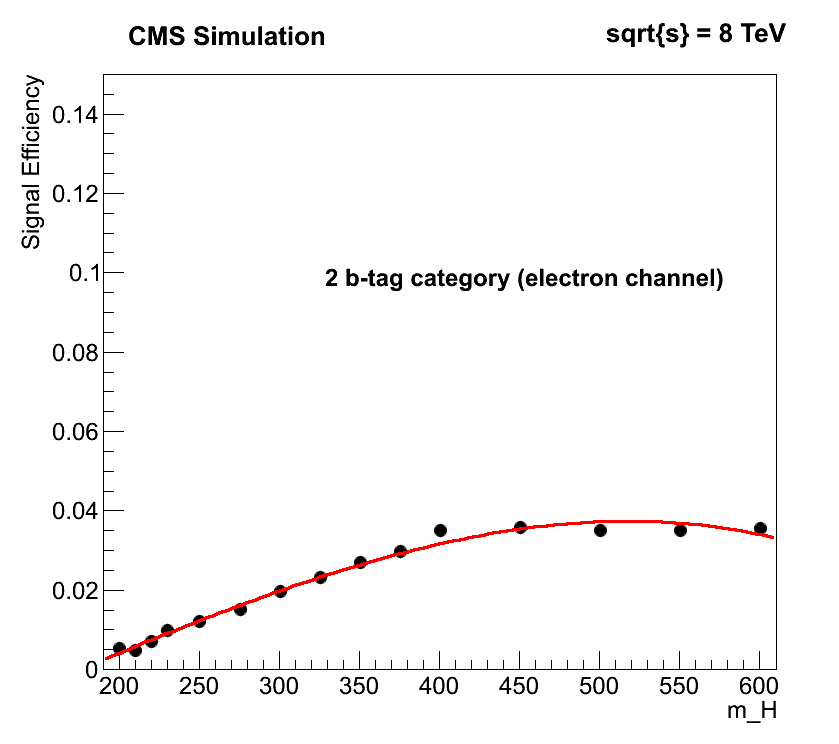
\includegraphics[width=0.3\textwidth]{images/plots/effFit_ELE_2btag.png}





%    Electrons\\
%    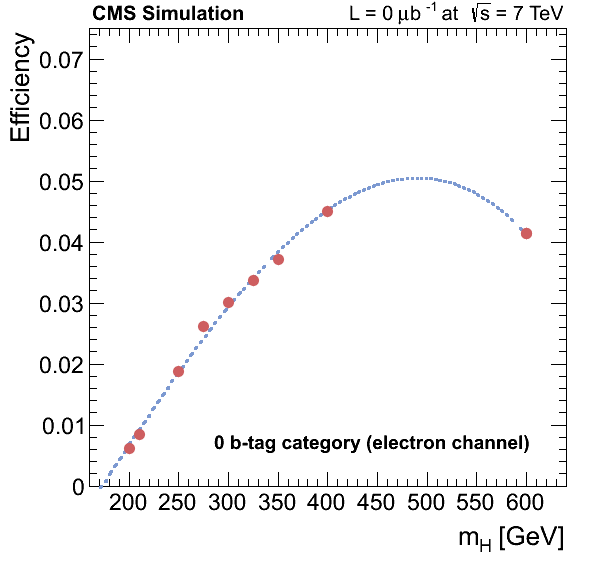
\includegraphics[width=0.3\textwidth]{images/fromDani/SignalEfficiencyFits27Sept_Run2012_AB/effFit_ELE_0btag.png}
%    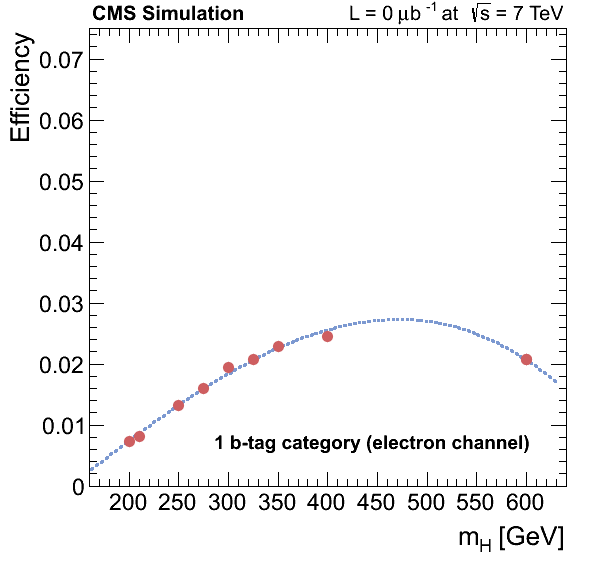
\includegraphics[width=0.3\textwidth]{images/fromDani/SignalEfficiencyFits27Sept_Run2012_AB/effFit_ELE_1btag.png}
%    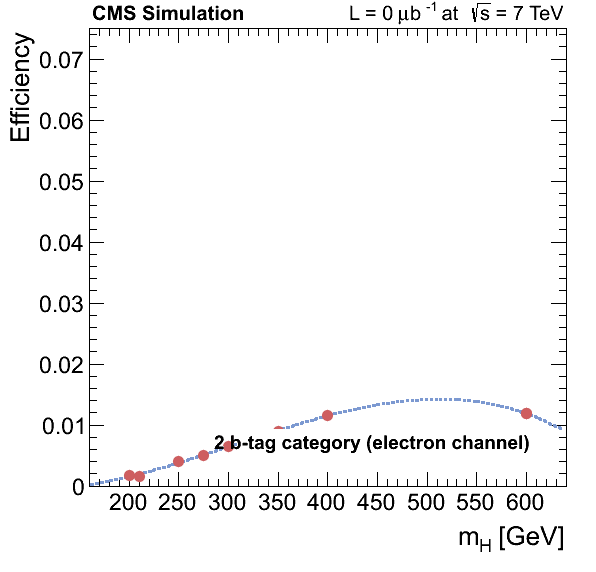
\includegraphics[width=0.3\textwidth]{images/fromDani/SignalEfficiencyFits27Sept_Run2012_AB/effFit_ELE_2btag.png}\\
%    Muons\\
%    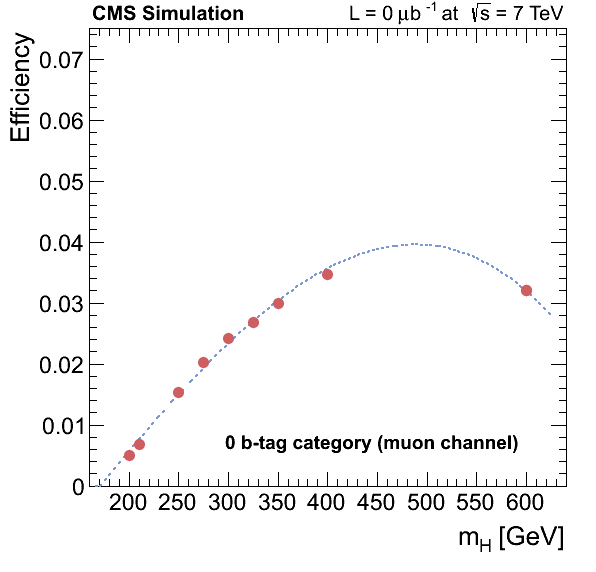
\includegraphics[width=0.3\textwidth]{images/fromDani/SignalEfficiencyFits27Sept_Run2012_AB/effFit_MU_0btag.png}
%    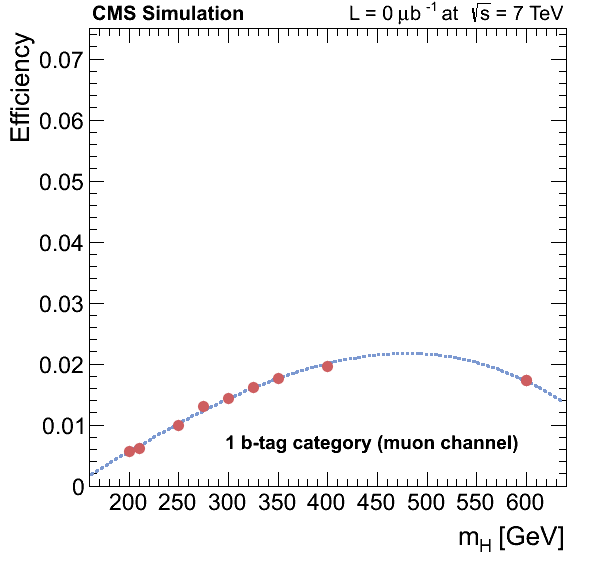
\includegraphics[width=0.3\textwidth]{images/fromDani/SignalEfficiencyFits27Sept_Run2012_AB/effFit_MU_1btag.png}
%    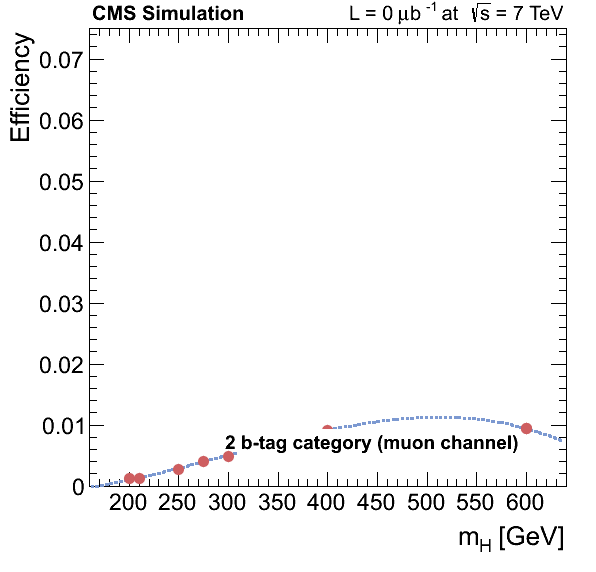
\includegraphics[width=0.3\textwidth]{images/fromDani/SignalEfficiencyFits27Sept_Run2012_AB/effFit_MU_2btag.png}

%\end{center}
%\end{frame}




\begin{frame}{Signal Systematics}
\begin{center}
%\footnotesize
%\scriptsize
%\tiny

\begin{tabular}{|l|c|c|c|}
%\begin{tabular}{|l|c|c|c|p{5cm}|}
\hline
Source      &   0 $b$-tag   &   1 $b$-tag  &   2 $b$-tag   \\ \hline \hline
Muon trigger \& ID               &  \multicolumn{3}{c|}{2.7\%}       \\
Electron trigger \& ID           &  \multicolumn{3}{c|}{2\%}         \\ \hline
Electron energy scale            &  \multicolumn{3}{c|}{0.2\%}       \\
Muon momentum scale              &  \multicolumn{3}{c|}{0.1\%}       \\ \hline
Jet reconstruction               &  \multicolumn{3}{c|}{1-4\%}       \\ \hline
$b$-tagging eff. and mistag rate &  1-4\% & 1-5\% & 5-8\%             \\ \hline
MET                              &  \multicolumn{3}{c|}{$<1$\%}       \\ \hline
Pile-up                          &  \multicolumn{3}{c|}{1-2\%}        \\
Production mechanism (PDF)       &  \multicolumn{3}{c|}{1.5\%}       \\
Production mechanism (lineshape) &  \multicolumn{3}{c|}{0-3\%}       \\
Luminosity                       &  \multicolumn{3}{c|}{4.4$\%$}      \\
Higgs cross-section              &  \multicolumn{3}{c|}{13-15$\%$ }  \\
\hline
\end{tabular}

%\begin{tabular}{|l|c|c|c|l|}
%\hline
%Source      &   0 $b$-tag   &   1 $b$-tag  &   2 $b$-tag  &   Comment \\ \hline \hline
%Muon trigger \& ID               &  \multicolumn{3}{c|}{2.7\%}       & Tag-\&-probe study \\
%Electron trigger \& ID           &  \multicolumn{3}{c|}{2\%}         & Tag-\&-probe study  \\ \hline
%Electron energy scale            &  \multicolumn{3}{c|}{0.2\%}       & \\
%Muon momentum scale              &  \multicolumn{3}{c|}{0.1\%}       & \\ \hline
%Jet reconstruction               &  \multicolumn{3}{c|}{1-4\%}       & JES, correlated among categories \\ \hline
%$b$-tagging eff. and mistag rate &  1-4\% & 1-5\% & 5-8\%            & Anti-correlated among categories \\ \hline
%MET                              &  \multicolumn{3}{c|}{$<1$\%}      & Loose requirement \\ \hline
%Pile-up                          &  \multicolumn{3}{c|}{1-2\%}       & Correlated between categories \\
%Production mechanism (PDF)       &  \multicolumn{3}{c|}{1.5\%}       & PDF4LHC, acceptance only\\
%Production mechanism (lineshape) &  \multicolumn{3}{c|}{0-3\%}       & Only for $M_H>400 GeV$  \\
%Luminosity                       &  \multicolumn{3}{c|}{4.4$\%$}     & Same for all analyses \\
%Higgs cross-section              &  \multicolumn{3}{c|}{13-15$\%$ }  & CERN Yellow Report   \\
%\hline
%\end{tabular}






\end{center}
\end{frame}

\begin{frame}{Background Systematics}
\begin{center}
\footnotesize
\begin{tabular}{|l|c|c|c|c|c|c|}
\hline
                           &   \multicolumn{3}{c|}{Normalization}   &   \multicolumn{3}{c|}{Shape}  \\ \hline
Source &   0 $b$-tag   &   1 $b$-tag  &   2 $b$-tag &   0 $b$-tag   &   1 $b$-tag  &   2 $b$-tag \\ \hline \hline
Muon trigger \& ID               &  \multicolumn{3}{c|}{2.7\%}            &    \multicolumn{3}{c|}{}      \\
Muon momentum scale              &  \multicolumn{3}{c|}{0.1\%}            &    \multicolumn{3}{c|}{}      \\
Electron trigger \& ID           &  \multicolumn{3}{c|}{2.0\%}            &    \multicolumn{3}{c|}{}      \\
Electron energy scale            &  \multicolumn{3}{c|}{0.5\%}            &     \multicolumn{3}{c|}{}     \\
Jet energy scale                 &  \multicolumn{3}{c|}{5.5\%}            &  \multicolumn{3}{c|}{0-4\%}  \\ 
\hline
$b$-tagging efficiency SF        & +0.4\% & -0.8\%  & -4.5\% &           \multicolumn{3}{c|}{} \\
Mistag SF                        & -1.9\% & +7.8\% & +6.2\%             &      \multicolumn{3}{c|}{}    \\ 
\hline
MET                              &  \multicolumn{3}{c|}{0.3\%}            &     \multicolumn{3}{c|}{}     \\ 
Pile-up                          &  \multicolumn{3}{c|}{0.1\%}            &     \multicolumn{3}{c|}{}     \\
$\pt^{\ell\ell jj}$ weighting       &  \multicolumn{3}{c|}{0.8\%}            &   \multicolumn{3}{c|}{0-3\%}  \\
Diboson cross section            &  \multicolumn{3}{c|}{15\%}             &     \multicolumn{3}{c|}{}     \\
Luminosity                       &  \multicolumn{3}{c|}{4.4\%}           &      \multicolumn{3}{c|}{}    \\ \hline 
Control Region                   &    \multicolumn{3}{c|}{}               &  0-15\% &  0-30\% &  0-40\%  \\
\hline 
\end{tabular} 
\end{center}
\end{frame}



\section{Results}


\begin{frame}{8 TeV Results}
\begin{center}
\scriptsize
\begin{columns}
\begin{column}{0.6\textwidth}
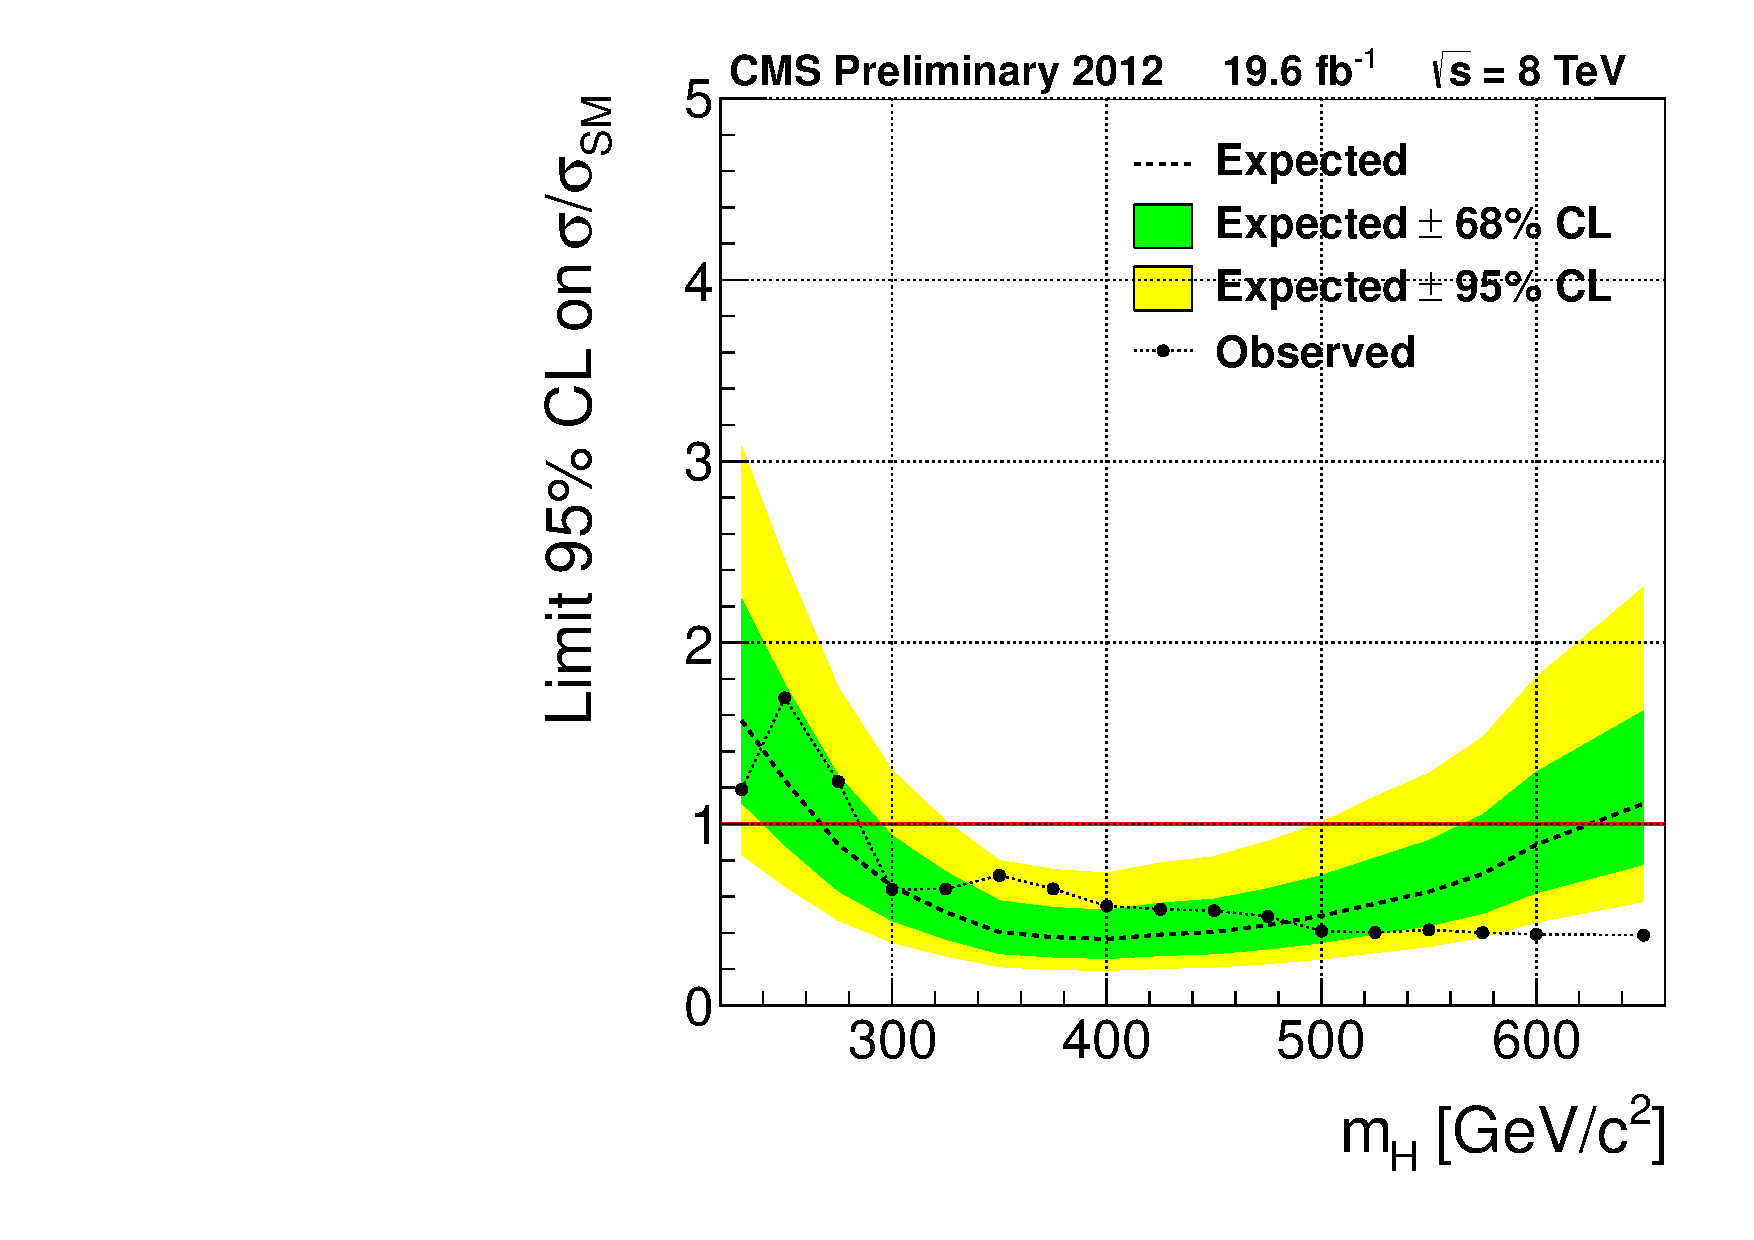
\includegraphics[width=1.0\textwidth]{images/8TeV_limit.pdf}
\end{column}
\begin{column}{0.4\textwidth}
Observed (solid) and expected (dashed) 95\% CL upper limit on the ratio of the production cross section to the SM expectation for the Higgs boson obtained using the $\mathrm{CL_s}$ technique.\\
\vspace{1em}
The 68\% and 95\% ranges of expectation for the background-only model are also shown with green and yellow bands, respectively.  The solid line at 1 indicates the expectation for a SM-Higgs-like boson.
\end{column}
\end{columns}
\end{center}
\end{frame}

\begin{frame}{8 TeV Individual Channel Results}
\begin{center}
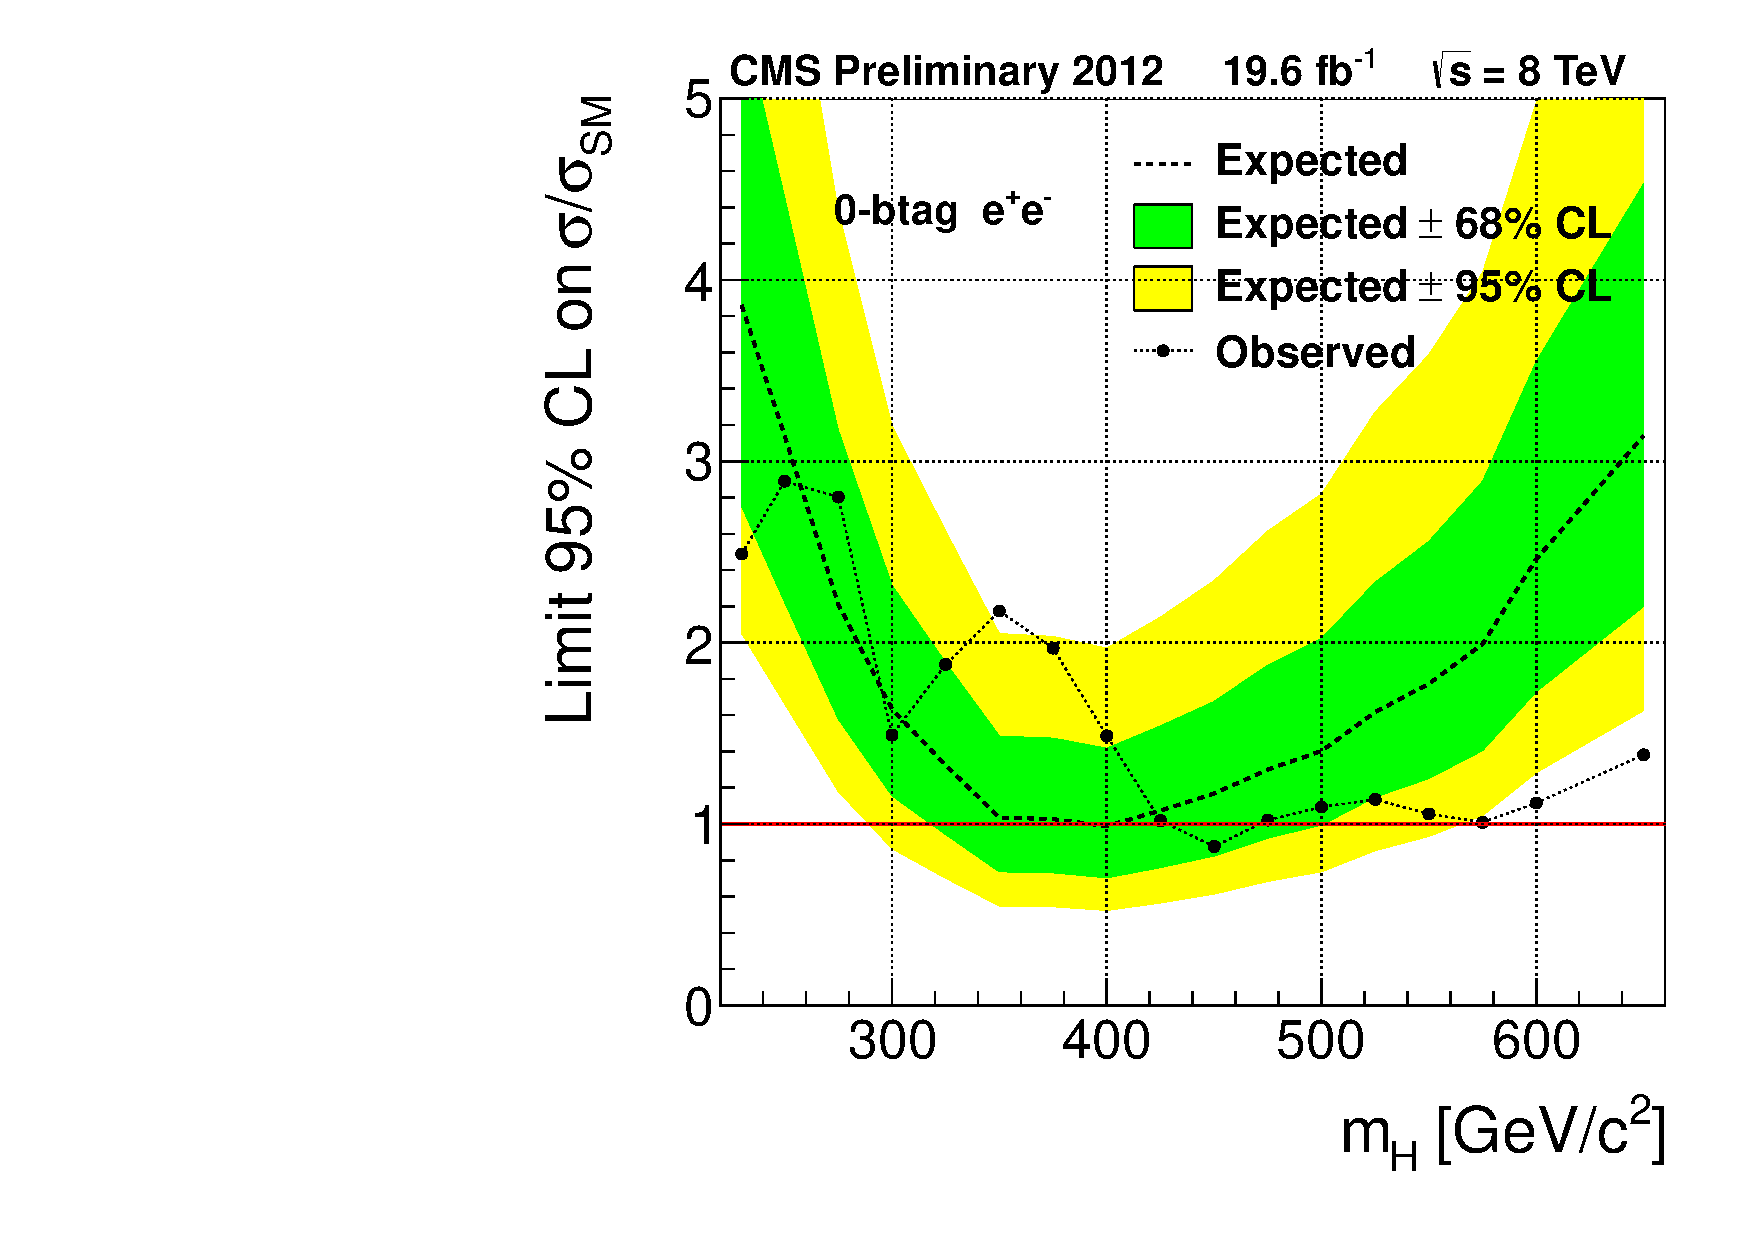
\includegraphics[width=0.33\textwidth]{images/limit_observed_0-btag_ee.pdf}
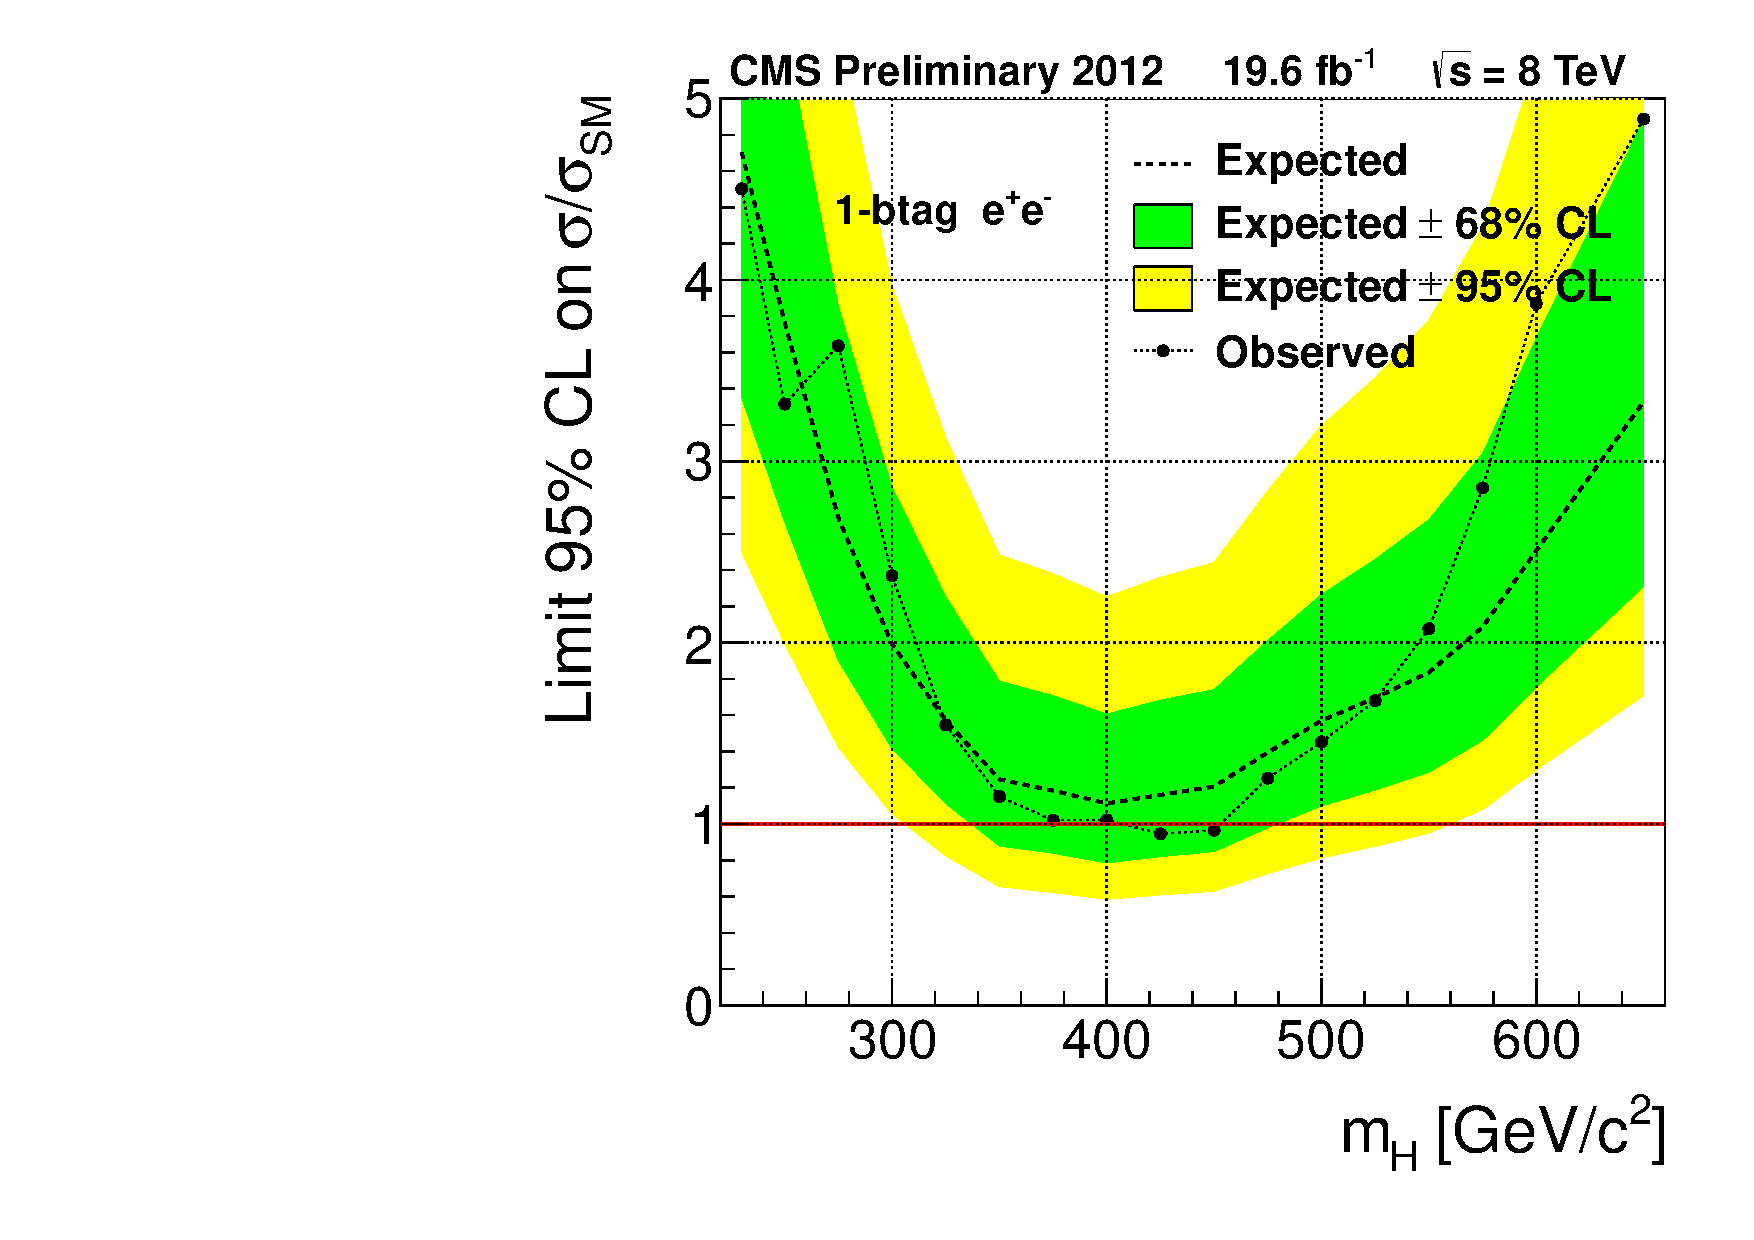
\includegraphics[width=0.33\textwidth]{images/limit_observed_1-btag_ee.pdf}
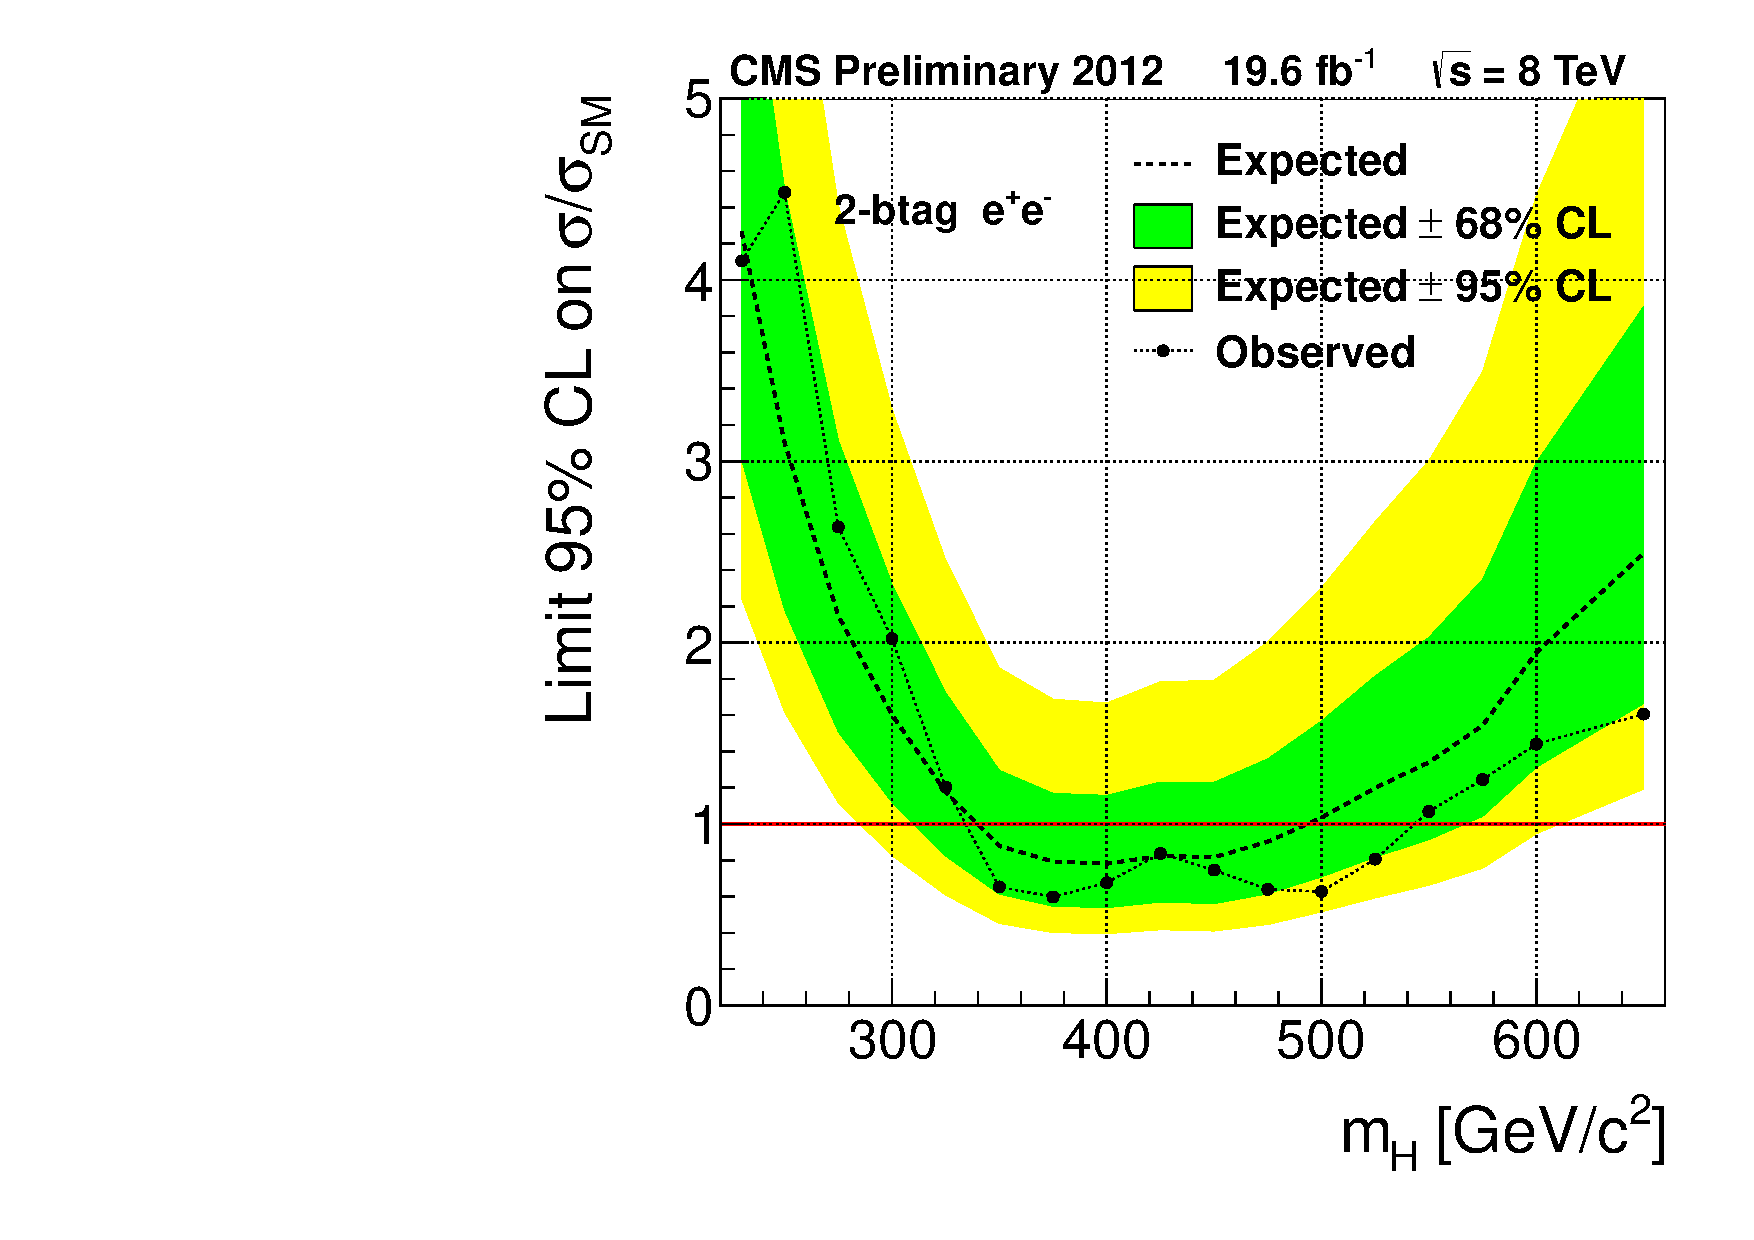
\includegraphics[width=0.33\textwidth]{images/limit_observed_2-btag_ee.pdf}\\
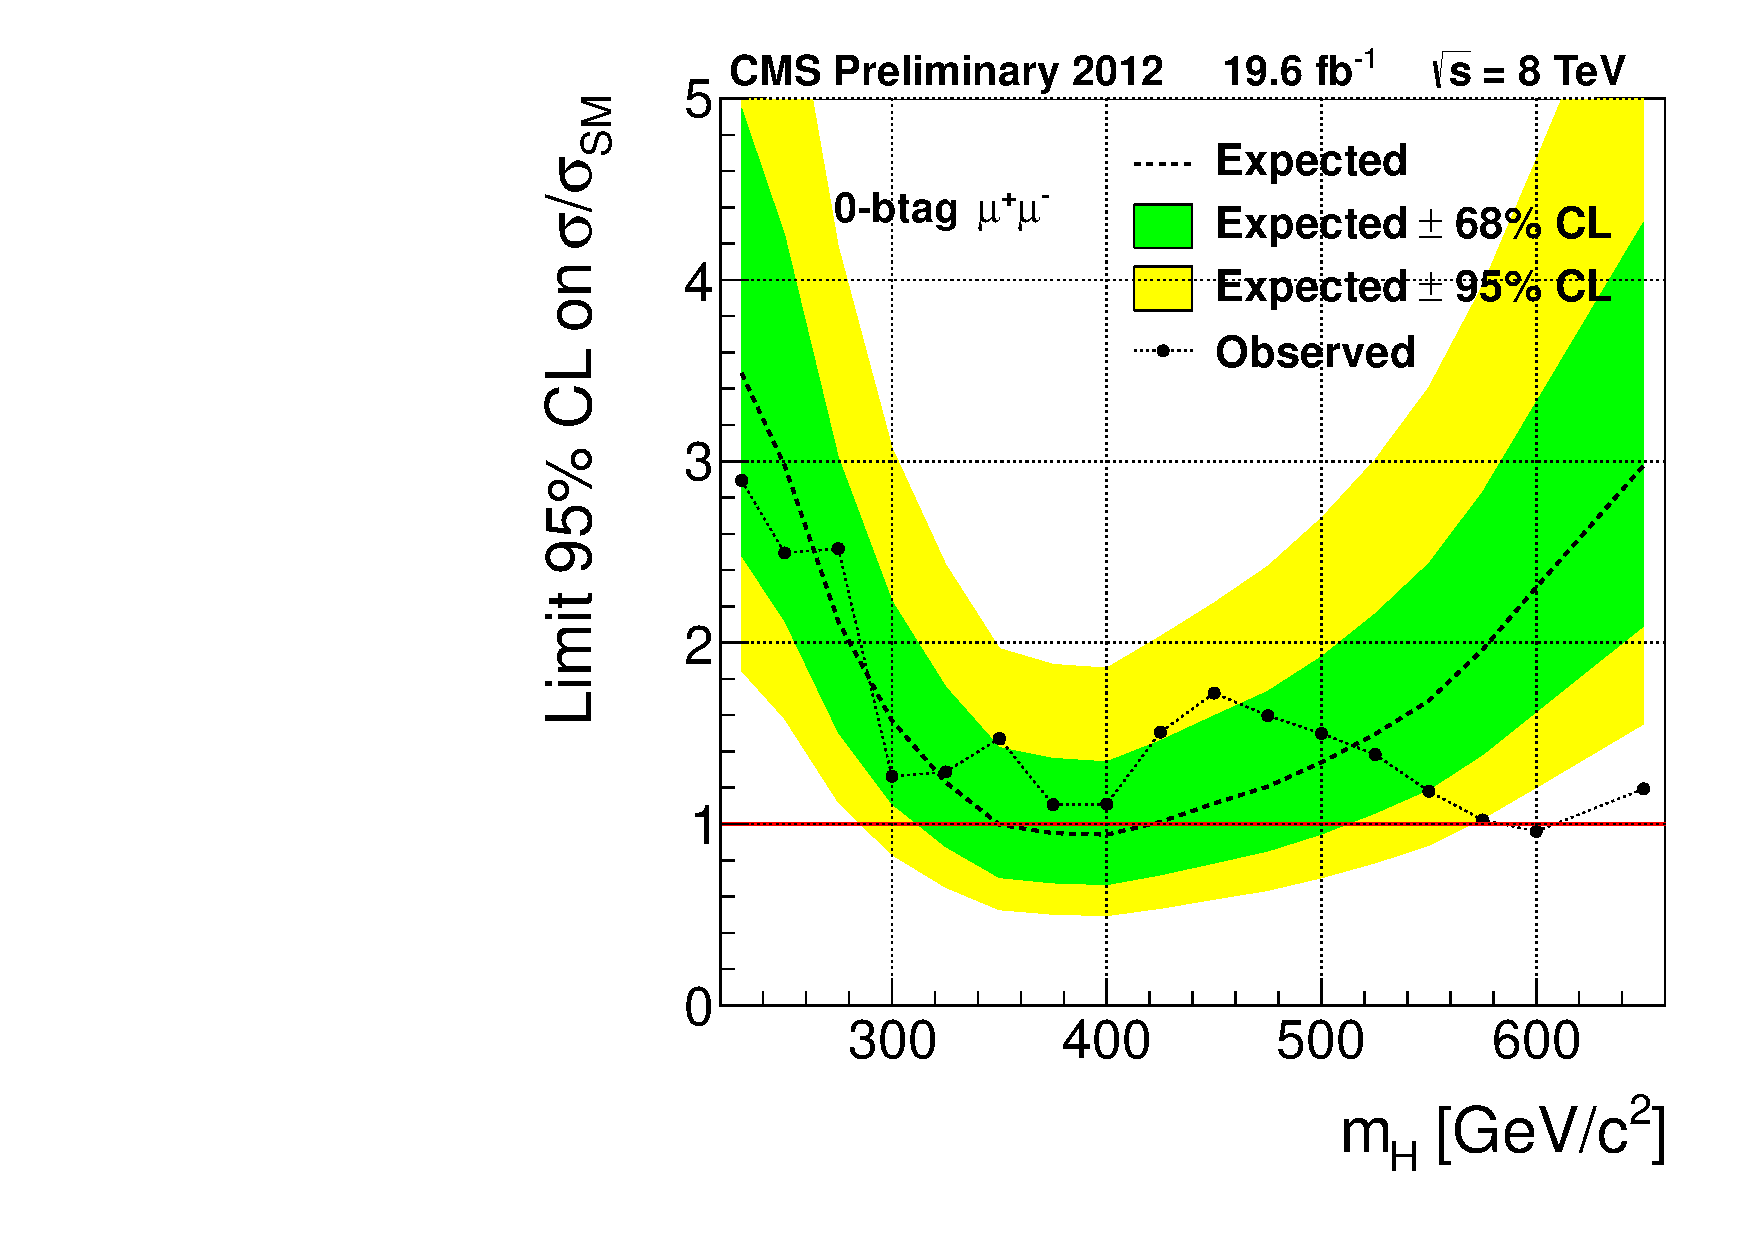
\includegraphics[width=0.33\textwidth]{images/limit_observed_0-btag_mm.pdf}
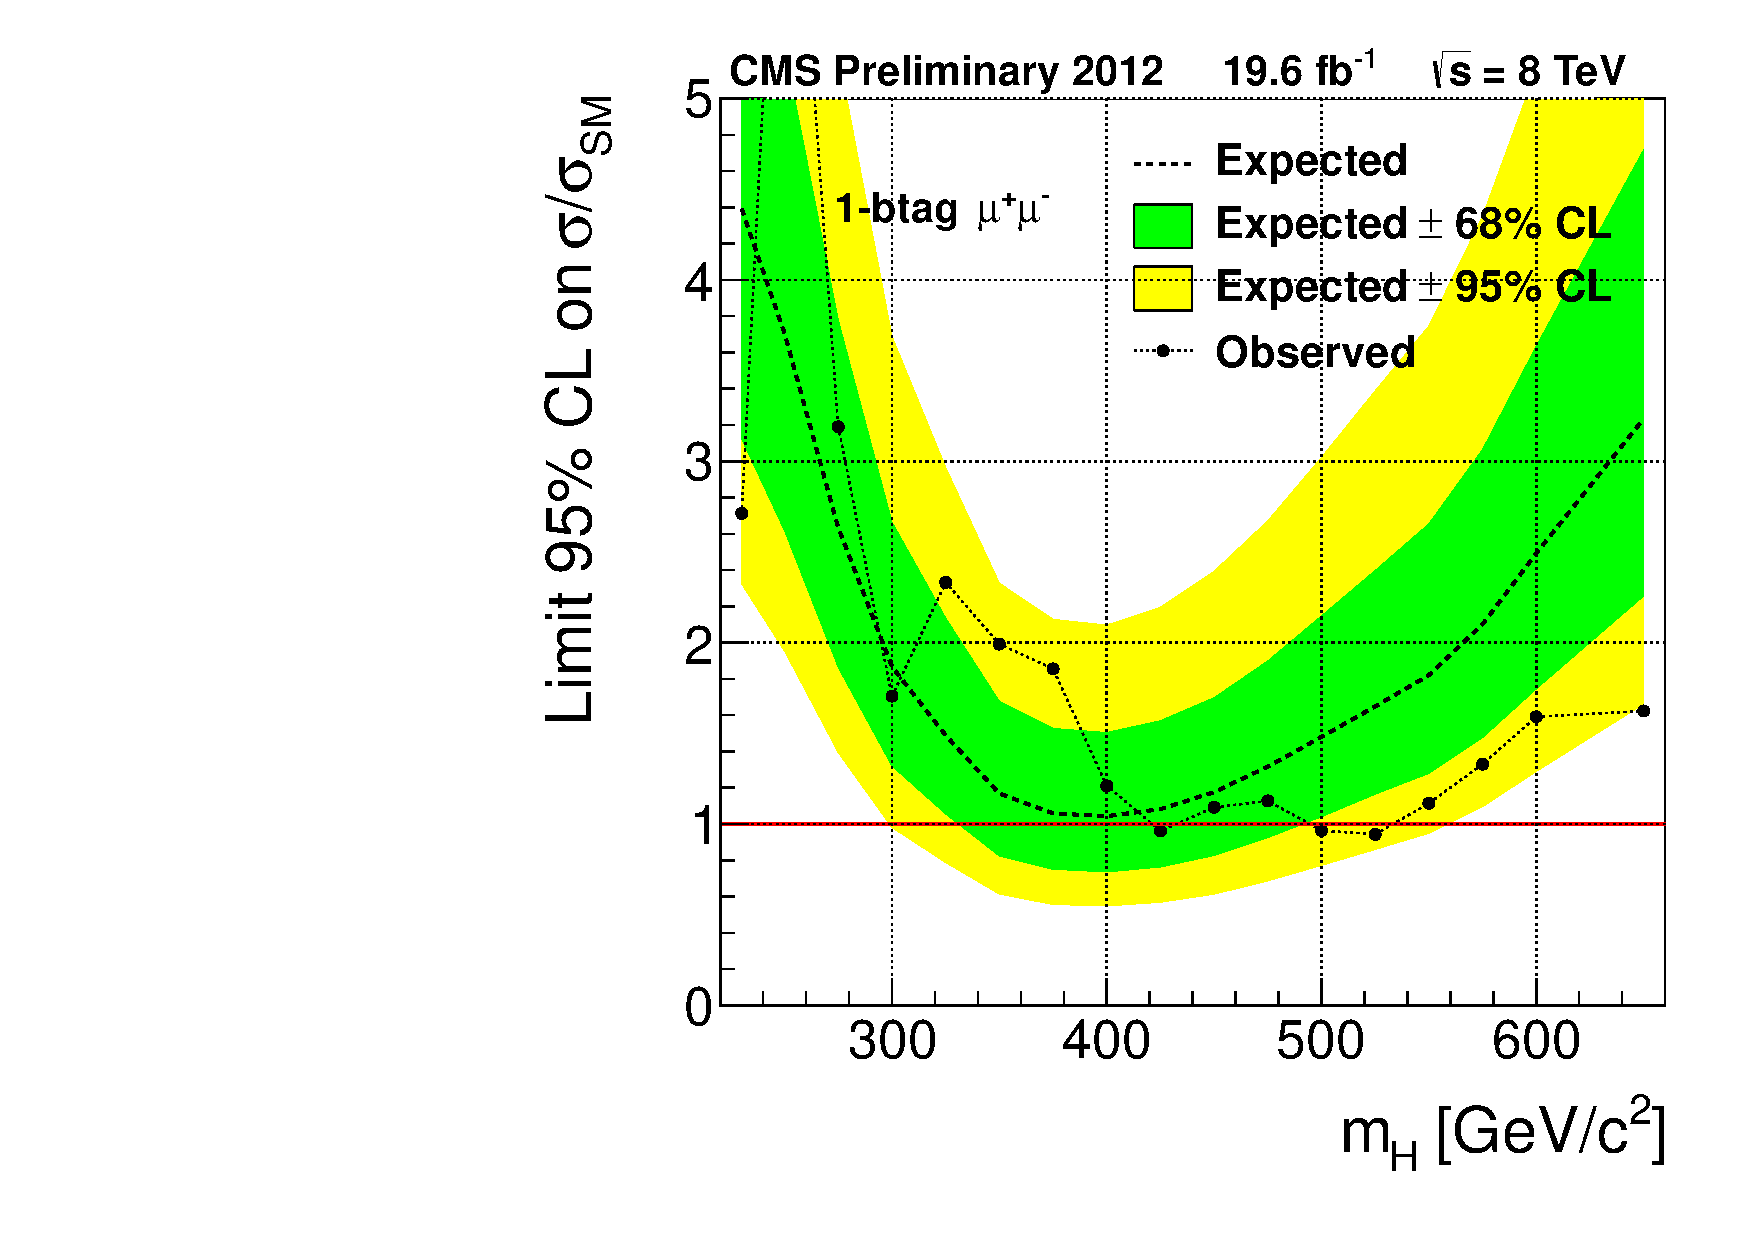
\includegraphics[width=0.33\textwidth]{images/limit_observed_1-btag_mm.pdf}
\includegraphics[width=0.33\textwidth]{images/limit_observed_2-btag_mm.pdf}\\
\end{center}
\end{frame}




\begin{frame}{HelyLD vs MLP}
\begin{center}
\scriptsize
%Limit on the expected 95$\%$ CL upper limit on the product of the Higgs boson production cross section and the branching fraction of H$\rightarrow$ZZ (dash line( and observed upper limit (black dots.) Yellow and Green bands represent the 68$\%$ and 95$\%$ ranges of expectation.
\begin{columns}
  \begin{column}{0.5\textwidth}
    \begin{center}
    {\large helyLD}\\ 
    \vspace{.2em}
   \includegraphics[width=1.\textwidth]{images/8TeV_limit.pdf}
   \end{center}
  \end{column}
  \begin{column}{0.5\textwidth}
    \begin{center}
    {\large MLP}\\
    \vspace{.2em}
    \includegraphics[width=1.\textwidth]{images/MVA_limit.pdf}
    \end{center}
  \end{column}
\end{columns}

\end{center}
%\vspace{.2em}
\footnotesize
The helyLD and MLP discriminators give very similar results, with the helyLD doing about 5\% better overall.  

\end{frame}




\begin{frame}{7 TeV and 8 TeV HelyLD Combined Results}
\begin{center}
\scriptsize
%Limit on the expected 95$\%$ CL upper limit on the product of the Higgs boson production cross section and the branching fraction of H$\rightarrow$ZZ (dash line( and observed upper limit (black dots.) Yellow and Green bands represent the 68$\%$ and 95$\%$ ranges of expectation.
\includegraphics[width=0.6\textwidth]{images/limit_observed_all-btag_combi.pdf}\\
\tiny
The 7 TeV 2l2q group results are in the backup slides.
\end{center}
\end{frame}

